\documentclass[11pt,a4paper]{article}

\usepackage{pifont}
\usepackage{amsmath}
\usepackage{amssymb}
% \usepackage{psfig}
\usepackage{graphicx}
\usepackage{array}
\usepackage{fancyheadings}
\usepackage{here}
\usepackage{pslatex}
\usepackage{eepic,epic}
\usepackage[english]{babel}
\usepackage[dvips,pageanchor=true,hyperindex=true,pagebackref=true,pdfhighlight=/O,pdfauthor={Yves Renard}]{hyperref}%pour le pdf

\usepackage{fancyheadings}
\usepackage{amsmath}
\usepackage{amssymb}
\usepackage{psfig}
\usepackage{here}
\usepackage{array}
\usepackage{alltt}
\usepackage{graphicx}
\usepackage{eepic,epic}
\usepackage[latin1]{inputenc}
\usepackage[T1]{fontenc}
% \usepackage[french]{babel}
% \usepackage[dvips]{epsfig}

%\oddsidemargin -0.2cm
%\evensidemargin -0.2cm
%\topmargin -1cm
%\textheight 22.5cm
%\textwidth 16.2cm
%\headheight 1.0cm

\newfont{\eufmtwelve}   {eufm10 scaled \magstep1}
\newfont{\eufmten}      {eufm10 }
\newfont{\eufmnine}     {eufm9 }
\newfont{\eufmeight}    {eufm8 }
\newfont{\eufmseven}    {eufm7 }
\newfont{\eufmsix}      {eufm6 }
\newfont{\eufmfive}     {eufm5 }
\newfont{\eusmtwelve}   {eusm10 scaled \magstep1}
\newfont{\eusmten}      {eusm10}
\newfont{\eusmnine}     {eusm9 }
\newfont{\eusmeight}    {eusm8 }
\newfont{\eusmseven}    {eusm7 }
\newfont{\eusmsix}      {eusm6 }
\newfont{\eusmfive}     {eusm5 }
\newfont{\msbmtwelve}   {msbm10 scaled \magstep1}
\newfont{\msbmeight}    {msbm8}

\newcommand{\udl}{\underline}
\newcommand{\udll}[1]{{\udl{\udl{#1}}}}
\newcommand{\udlll}[1]{{\udl{\udl{\udl{#1}}}}}
\newcommand{\mat}[1]{{\mbox{\msbmtwelve {#1}}}}
\newcommand{\Reel}{{\mbox{\msbmtwelve R}}}      % L'ensemble des reels.
\newcommand{\reel}{{\mbox{\msbmeight R}}}       % L'ensemble des reels.
%\newcommand{\Reel}{{\rm I\hspace{-0.15em}R}}
\newcommand{\Complex}{\mbox{\msbmtwelve C}}     % L'ensemble des complexes.
\newcommand{\Naturel}{\mbox{\msbmtwelve N}}  % L'ensemble des entiers naturels.
\newcommand{\naturel}{\mbox{\msbmeight N}}   % L'ensemble des entiers naturels.

%\newcommand{\Naturel}{{\rm I\hspace{-0.15em}N}}% L'ensemble des entiers naturels.
\renewcommand{\emptyset}{\mbox{$\circ$\hspace{-.50em}/}}  % ensemble vide.
\newcommand{\Cont}{{\cal C}}            % L'ensemble des fonctions continues
\newcommand{\Cinf}{{\cal C}^{\infty}}   % L'ensemble des fonction C-infinies
\renewcommand{\vec}[1]{\overrightarrow{\!\!#1}}
\newcommand{\subsetcont}{{\subset\hspace{-.6em}_{\scriptscriptstyle >} }}
\newcommand{\Frac}[2]{{\ds \frac{\ds #1}{\ds #2}}}
\newcommand{\interior}[1]{{\stackrel{\circ}{#1}}}
\newcommand{\cqfd}{{$\mbox{}$\hfill\rule{2.5mm}{2.5mm}}}
\newcommand{\vectwo}[2]{{\left(\hspace{-.5em}\begin{array}{c} {#1} \\ {#2}
     \end{array}\hspace{-.5em}\right)}}
\newcommand{\vecthree}[3]{{\left(\hspace{-.5em}\begin{array}{c} {#1}
     \\ {#2} \\ {#3} \end{array}\hspace{-.5em}\right)}}
\newcommand{\vecfour}[4]{{\left(\hspace{-.5em}\begin{array}{c} {#1}
     \\ {#2} \\ {#3} \\ {#4} \end{array}\hspace{-.5em}\right)}}
\newcommand{\vecfive}[5]{{\left(\hspace{-.5em}\begin{array}{c} {#1}
     \\ {#2} \\ {#3} \\ {#4} \\ {#5} \end{array}\hspace{-.5em}\right)}}
\newcommand{\vecseven}[7]{{\left(\hspace{-.5em}\begin{array}{c} {#1}
     \\ {#2} \\ {#3} \\ {#4} \\ {#5} \\ {#6} \\ {#7} \end{array}\hspace{-.5em}\right)}}
\def\infess{\mathop{\iflanguage{english}{\mbox{ess$\,$inf}}{\mbox{inf$\,$ess}}}}
\def\supess{\mathop{\iflanguage{english}{\mbox{ess$\,$sup}}{\mbox{sup$\,$ess}}}}
\def\essinf{\mathop{\iflanguage{english}{\mbox{ess$\,$inf}}{\mbox{inf$\,$ess}}}}
\def\esssup{\mathop{\iflanguage{english}{\mbox{ess$\,$sup}}{\mbox{sup$\,$ess}}}}
\def\aplim{\mathop{\mbox{ap$\,$lim}}}
\def\aplimsup{\mathop{\mbox{ap$\,$lim$\,$sup}}}
\def\apliminf{\mathop{\mbox{ap$\,$lim$\,$inf}}}
\def\convto{\mathop{\hbox{\rightarrowfill}}} % converge vers.
\newcommand{\rightgap}{{]\hspace{-0.12em}]}}
\newcommand{\leftgap}{{[\hspace{-0.12em}[}}
\newcommand{\gapof}[1]{{\leftgap {#1} \rightgap}}
\newcommand{\restrictiona}[1]
{{ \begin{picture}(13,10) \put(-1,-4){$\mid_{#1}$} \end{picture}
}} % Le signe "Restriction sur #1"

\def\Indic{\mbox{1\hspace{-0.20em}I}}   % Fonction l'indicatrice

% \def\bar3{|\hspace{-1pt}\|} % 3bar verticaux pour les normes matricielles.
\def\cvweak{\mathop{-\hspace{-0.3em}-\hspace{-0.6em}\rightharpoonup}} % fleche cv faible
\def\cvweakstar{\cvweak^*} % fleche cv faible etoile
\def\longmapsto
{ \begin{picture}(0,10)
  \put(0,0){$\scriptstyle{\vdash}$} \end{picture} \mbox{$\longrightarrow$}
} 

\def\build#1_#2^#3{\mathrel{
 \mathop{\kern 0pt#1}\limits_{#2}^{#3}}} % Ecrire en dessous et dessus un symbole.

\def\Dist{\mbox{\eusmtwelve D}} %signe de distribution
\def\dist{\mbox{\eusmten D}} %signe de distribution


%definition de commandes utilises
\newcommand{\ds}{\displaystyle}
\newcommand{\rc}{{\par}}
\newcommand{\rcc}{{\par\medskip}}
\newcommand{\rccc}{{\par\bigskip}}


%definition des environnements theoreme, lemme, ...
\usepackage{boxedminipage}
% \newenvironment{largebox}
%   { \rc\noindent \begin{boxedminipage}[t]{\textwidth} }
%   { \end{boxedminipage}  \rccc\noindent }
\newenvironment{largebox}
  { \rc\noindent \begin{boxedminipage}[t]{\linewidth} }
  { \end{boxedminipage}  \rccc\noindent }


\newtheorem{ltheoreme}{Th\'eor\`eme}
\newenvironment{theoreme}
  { \begin{largebox} \begin{ltheoreme} }
  { \end{ltheoreme} \end{largebox} }
\newtheorem{lproposition}{Proposition}
\newenvironment{proposition}
  { \begin{largebox} \begin{lproposition} }
  { \end{lproposition} \end{largebox} }
\newtheorem{llemme}{Lemme}
\newenvironment{lemme}
  { \begin{largebox} \begin{llemme} }
  { \end{llemme} \end{largebox} }
\newtheorem{ldefinition}{D\'efinition}
\newenvironment{definition}
  { \begin{largebox} \begin{ldefinition} }
  { \end{ldefinition} \end{largebox} }
\newtheorem{lhypothese}{Hypoth\`ese}
\newenvironment{hypothese}
  { \begin{largebox} \begin{lhypothese} }
  { \end{lhypothese} \end{largebox} }
\newtheorem{lcorollaire}{Corollaire}
\newenvironment{corollaire}
  { \begin{largebox} \begin{lcorollaire} }
  { \end{lcorollaire} \end{largebox} }
\newenvironment{remarque}
  { \begin{largebox} {\bf \udl{Remarque} : }}
  { \end{largebox} }

\newcounter{numberofprobl}
\setcounter{numberofprobl}{1}

\newlength{\compteurtpourprobla}
\newlength{\compteurtpourproblb}
\newenvironment{caseeqnarray}[1]
  {
   $${#1}
   \settowidth{\compteurtpourprobla}{${#1}\left\{\right.$}
   \setlength{\compteurtpourproblb}{\textwidth}
   \addtolength{\compteurtpourproblb}{-1\compteurtpourprobla}
   \settowidth{\compteurtpourprobla}{$\;$}
   \addtolength{\compteurtpourproblb}{-1\compteurtpourprobla}
   \left\{ \begin{minipage}[l]{\compteurtpourproblb}
   \vspace{-1em} \begin{eqnarray}
  }
  { \end{eqnarray} \end{minipage} \right. $$}


\newtheorem{hypothesis}{Hypothesis}
\newtheorem{prop}{Proposition}
\newtheorem{defi}{Definition}
%\newtheorem{theorem}{Theorem}
%\newtheorem{lemma}{Lemma}


% pour plus tard ...
% \DeclareGraphicsRule{ps.Z}{eps}{ps.bb}{`zcat #1}
% \DeclareGraphicsRule{eps.Z}{eps}{eps.bb}{`zcat #1}
% \DeclareGraphicsRule{ps.gz}{eps}{ps.bb}{`gunzip #1}
% \DeclareGraphicsRule{eps.gz}{eps}{eps.bb}{`gunzip #1}


\oddsidemargin -0.9cm
\evensidemargin -0.9cm
\topmargin -2cm
\textheight 24.5cm
\textwidth 17.6cm
\headheight 1.0cm

% principal notations



\begin{document}

\begin{center}
  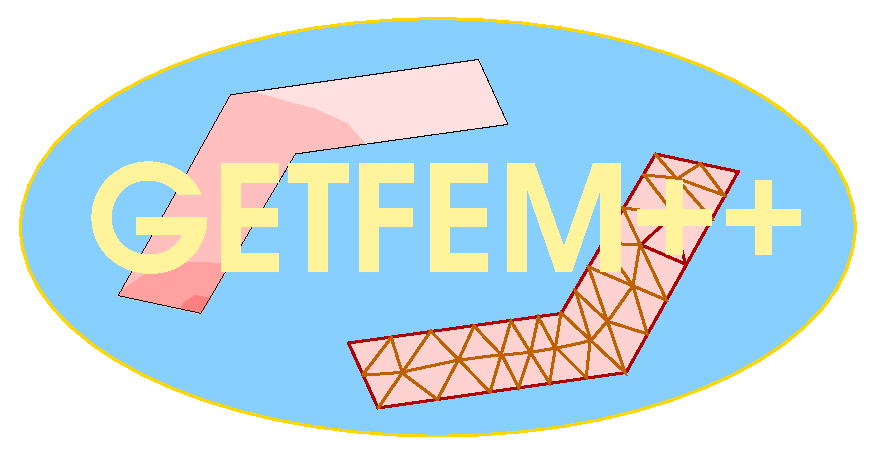
\includegraphics[width=10cm,angle=0]{getfem_logo.eps}\\[0.2cm]
  a Generic Finite Element library in C++ \\[0.5cm]
  {\LARGE Documentation, part \Huge 3} \\[0.5cm]
  \begin{largebox} \begin{center}
      \Huge \sc Description of Finite Element and Integration Methods
  \end{center}  \end{largebox}
  \\[0.5cm]
  { \large Yves \sc Renard\footnote{ \it MIP, INSAT, Complexe scientifique de Rangueil, 31077 Toulouse, France, Yves.Renard@insa-toulouse.fr }, Julien Pommier\footnote{ \it MIP, INSAT, Complexe scientifique de Rangueil, 31077 Toulouse, France, Julien.Pommier@insa-toulouse.fr } } \\[1.0cm]
      \today \\[1.0cm]
\end{center}

% \begin{abstract}
% Basic description of the structure of the finite element kernel of {\sc Getfem++}.
% \end{abstract}


%%%%%%%%%%%%%%%%%%%%%%%%%%%%%%%%%%%%%%%%%%%%%%%%%%%%%%%%%%%%%%%%%%%%%%%%%
%          INTRODUCTION                                                 %
%%%%%%%%%%%%%%%%%%%%%%%%%%%%%%%%%%%%%%%%%%%%%%%%%%%%%%%%%%%%%%%%%%%%%%%%%

\section*{Introduction}
This documentation describes the different finite element methods and approximative integration methods available in {\sc Getfem++}.\\[5cm]
Copyright (C) 2000-2020 Yves Renard, Julien Pommier.\\
The program GetFEM is free software; you can redistribute it and/or modify
it under the terms of the GNU Lesser General Public License as published by
the Free Software Foundation; either version 3 of the License, or
(at your option) any later version along with the GCC Runtime Library
Exception either version 3.1 or (at your option) any later version.
This program is distributed in the hope that it will be useful,
but WITHOUT ANY WARRANTY; without even the implied warranty of
MERCHANTABILITY or FITNESS FOR A PARTICULAR PURPOSE.  See the
GNU Lesser General Public License for more details.
You should have received a copy of the GNU  Lesser General Public License
along with this program; if not, write to the Free Software Foundation,
Inc., 51 Franklin Street, Fifth Floor, Boston, MA  02110-1301  USA

\newpage
\tableofcontents
\newpage

\section{Finite element methods}

All finite element methods defined in {\sc Getfem++} are interfaced in the file {\tt getfem\_fem.h}.
A descriptor on a finite element method is available thanks to the function\\[0.5cm]
{\tt getfem::pfem pf = getfem::fem\_descriptor("name of method");
}\\[0.5cm]
where {\tt "name of method"} is a string to be choosen among the existing methods.

\subsection{Finite element methods description}

\begin{figure}[H]
  \begin{center} 
    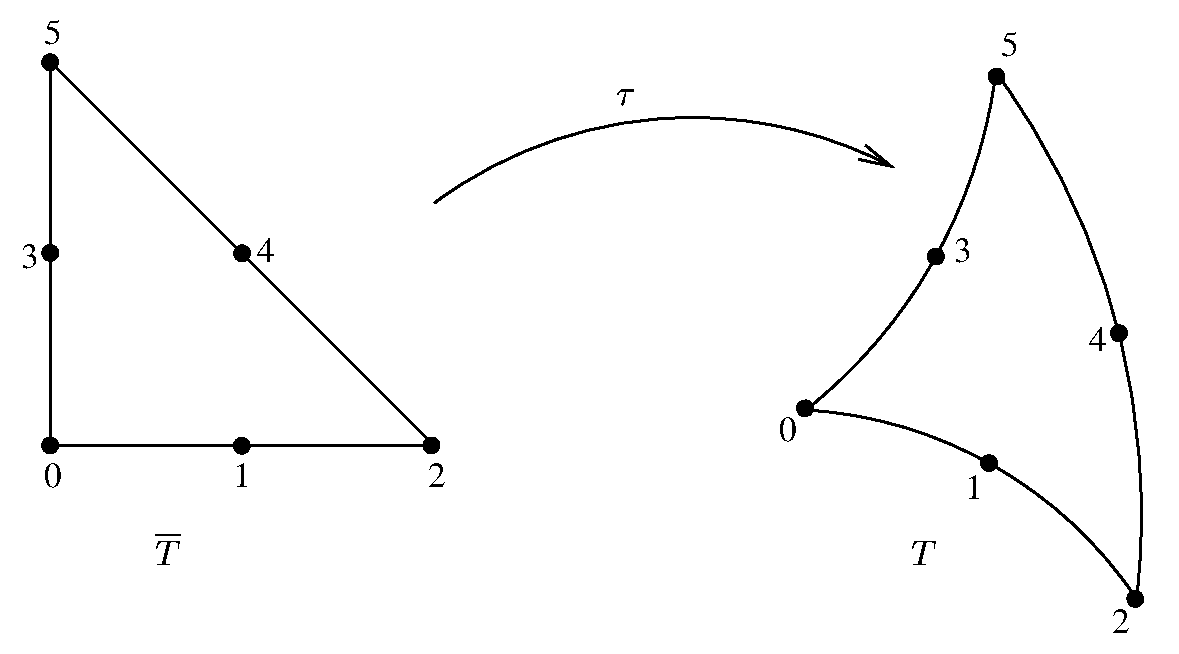
\includegraphics[width=12cm,angle=0]{getfemlist_extrans.eps}
    \caption{ \it Example of geometric transformation for a triangle.} \label{fig:extrans}
  \end{center}
\end{figure}

A finite element method is defined on a reference element $\hat{T} \subset \Reel^P$ by a set of $n_d$ nodes $a^i$ and corresponding base functions 
$$ \hat{\varphi}^i : \hat{T} \subset \Reel^P \longrightarrow \Reel^Q. $$
Each base function corresponds to a degree of freedom (d.o.f).
Most finite element methods are scalar, which means that $Q = 1$, but {\sc Getfem++} support also intrinsic vectorial elements. The map between the reference element and the real element is called the geometric transformation and is denoted by 
$$ \tau :  \hat{T} \longrightarrow T, $$
and is supposed to be polynomial (see \cite{dh-to1984} or \cite{BAS_COMP}). The base functions $\hat{\varphi}^i$ defined on the reference element define a set of base function on the real element defined by
$$ \tilde{\varphi}^i(x) = \hat{\varphi}^i(\hat{x}) = \hat{\varphi}^i(\tau^{-1}(x)), $$
If the element is said to be equivalent throught the geometric transformation $\tau$ (or $\tau$-equivalent) then base functions on the real element are just defined by
$$\varphi^i(x) = \tilde{\varphi}^i(x).$$
This is generally the case for Lagrange element, but not for Hermite elements (when some dof represent the gradient of the unkown). When the element is not equivalent throught the geometric transformation then {\sc Getfem++} allows to define a matrix $\tilde{M}$ depending on the real element (i.e. on the geometric transformation) such that base functions on the real element are defined by
$$ \varphi^i(x) = \sum_{j = 0}^{n_d - 1} \tilde{M}_{ij} \tilde{\varphi}^j(x). $$
Most of the time, the matrix $\tilde{M}$ is a square matrix, but for special elements a non-square matrix can be defined.
We denote by
$$ [\hat{\varphi}(\hat{x})] = \vecfour{\hat{\varphi}^0(\hat{x})}{\hat{\varphi}^1(\hat{x})}{...}{\hat{\varphi}^{n_d-1}(\hat{x})}, $$
the $n_d \times Q$ matrix, such that when a function is defined by
$$ f(x) = \sum_{i = 0}^{n_d - 1} \alpha_i \varphi^i(x), $$
one has
$$ \hspace{1em} f(\tau(\hat{x})) = \alpha^T \tilde{M} [\hat{\varphi}(\hat{x})],\hspace{1em} $$
where $\alpha$ is the vector of components $\alpha_i$.

\subsubsection{Different types of d.o.f.}

To each base function of a finite element method corresponds a degree of freedom (d.o.f) which is a linear form on this function. The following table gives the most significant types of d.o.f.\\

\begin{center}
\begin{tabular}{|m{3cm}|m{3cm}|m{8cm}|} \hline 
type & expression  & commentary \\ \hline
\end{tabular}
\begin{tabular}{|m{3cm}|m{3cm}|m{8cm}|} \hline
Lagrange type & $\phi(a_i)$ & Value of $\phi$ on the node $a_i$. The most simple d.o.f. Allows the Lagrange interpolation. \\ \hline
\end{tabular}
\begin{tabular}{|m{3cm}|m{3cm}|m{8cm}|} \hline
Hierarchical ~~~~~~~ Lagrange type & $\phi(a_i) - ...$ & Difference between the value of $\phi$ on the node $a_i$ and the value of some other base functions. This is generally the bubble functions type of d.o.f . \\ \hline
\end{tabular}
\begin{tabular}{|m{3cm}|m{3cm}|m{8cm}|} \hline
mean type & $\Frac{1}{|T|}\ds \int_T \phi(x) dx$ & Value of the mean value of $\phi$ on the element. Exists also for the restriction on a face.\\ \hline
\end{tabular}
\begin{tabular}{|m{3cm}|m{3cm}|m{8cm}|} \hline
derivative type & $\Frac{\partial}{\partial x_i}\phi(a_i)$ or $\Frac{\partial}{\partial n}\phi(a_i)$ & Value of a derivative of $\phi$ on the node $a_i$. This kind of d.o.f. makes the element not to be $\tau$-equivalent. $\Frac{\partial}{\partial n}\phi(a_i)$ denotes the normal derivative with respect to a face.\\ \hline
\end{tabular}
\begin{tabular}{|m{3cm}|m{3cm}|m{8cm}|} \hline
second derivative type & $\Frac{\partial^2}{\partial x_i\partial x_j}\phi(a_i)$  & Value of a second derivative of $\phi$ on the node $a_i$. This kind of d.o.f. makes also the element not to be $\tau$-equivalent.\\ \hline
\end{tabular}

\end{center}

\subsubsection{Graphical codification of d.o.f.}

\begin{figure}[H] \label{fig:symbols}
  \begin{center}
    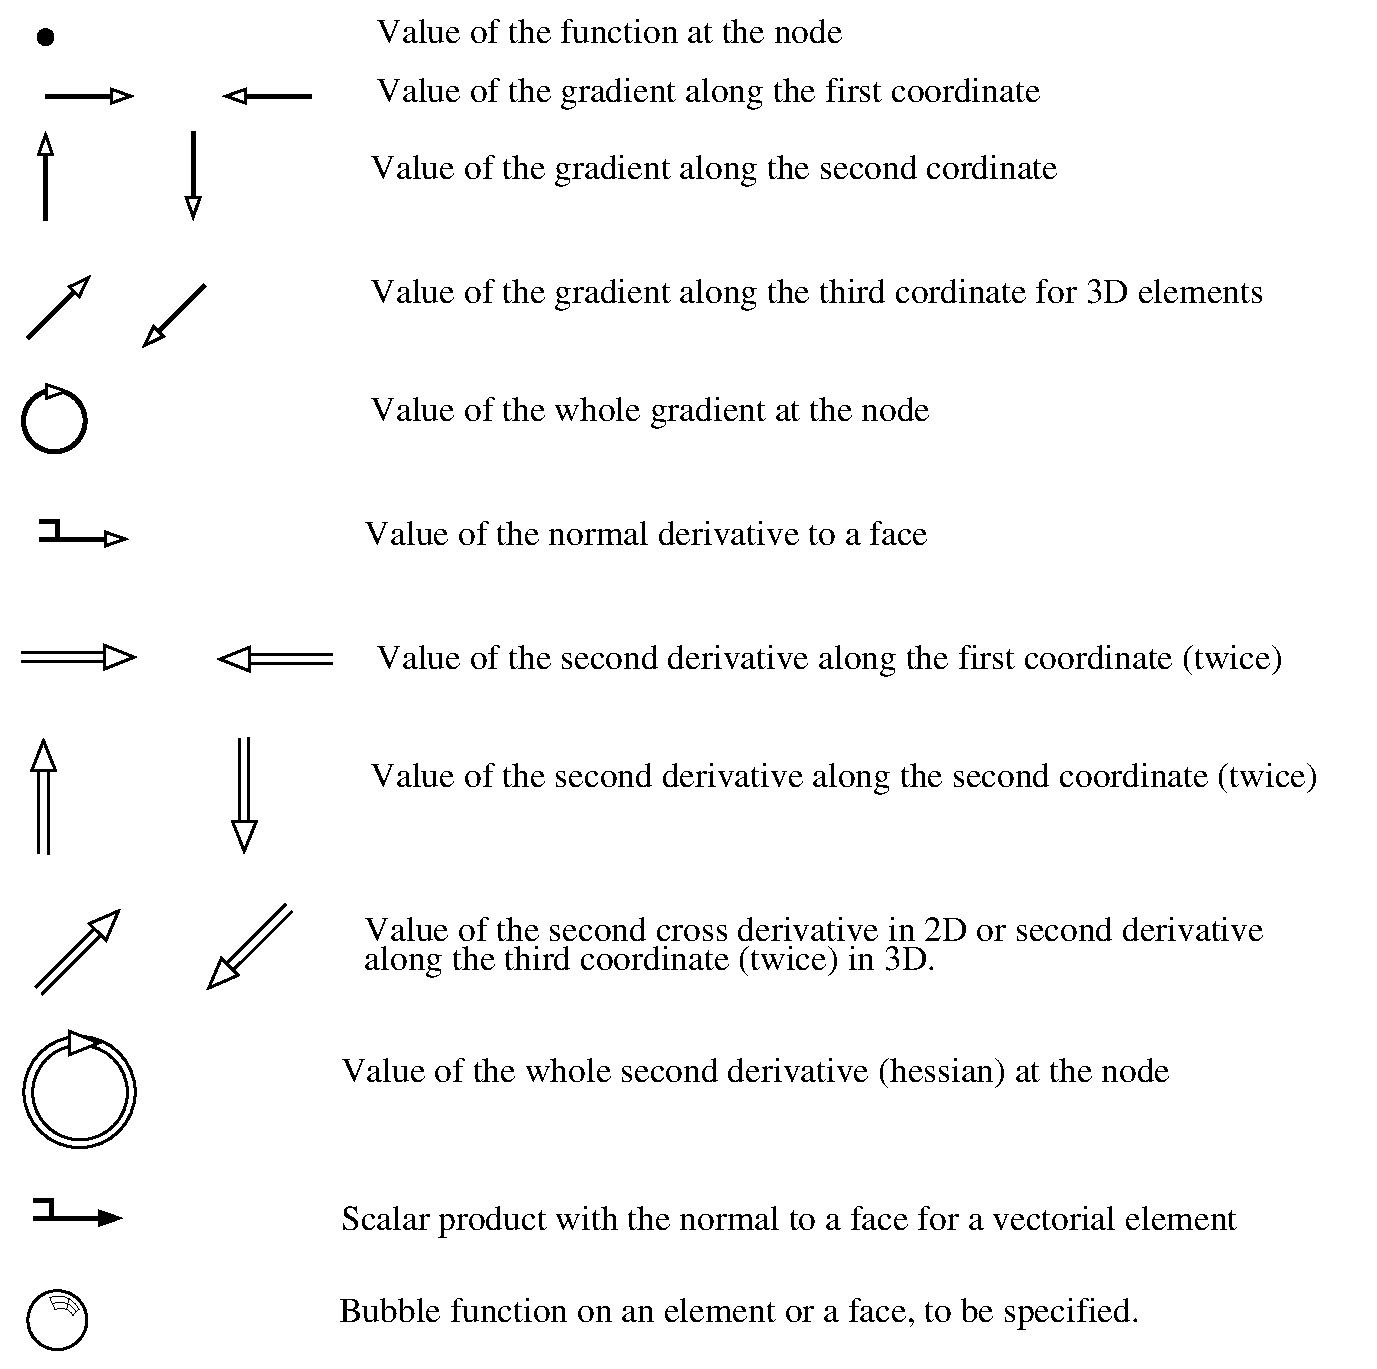
\includegraphics[width=13cm,angle=0]{getfemlist_symbols.eps}
  \end{center}
  \caption{ \it Symbols representing degree of freedom types}
\end{figure}

% a chaque {\'e}l{\'e}ment : 
% dessin des ddl avec code
% nb de ddl, degre, equivalence via la transformation g{\'e}ometrique, vectoriel ou non, analyse du raccord

\subsection{Classical ``$P_K$'' Lagrange elements on simplices}

It is possible to define a classical ``$P_K$'' Lagrange element of arbitrary dimension and arbitrary degree. This element has only degrees of freedom which corresponds to the value of the function on a node. The grid of node is the so-called Lagrange grid. Figures \ref{fig:segmentpk}, \ref{fig:trianglepk} and \ref{fig:tetrahedronpk} show examples of dimension 1, 2 and 3.
\begin{figure}[H] 
  \begin{center} 
    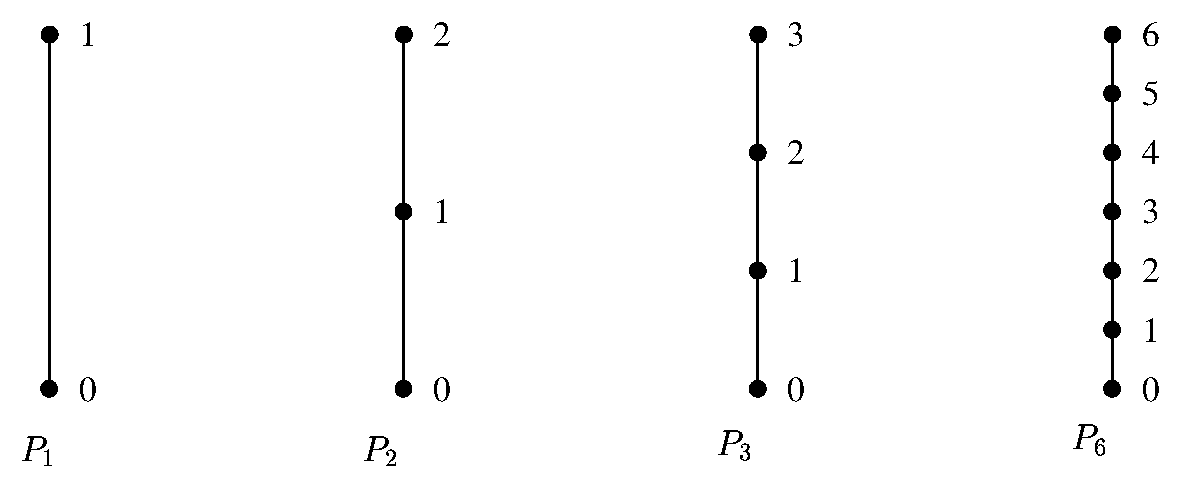
\includegraphics[width=14cm,angle=0]{getfemlist_segment_Pk.eps}
    \caption{ \it Examples of classical $P_K$ Lagrange elements on a segment.} \label{fig:segmentpk}
  \end{center}
\end{figure}
\begin{figure}[H]
  \begin{center} \begin{tabular}{m{7cm}m{7cm}}
    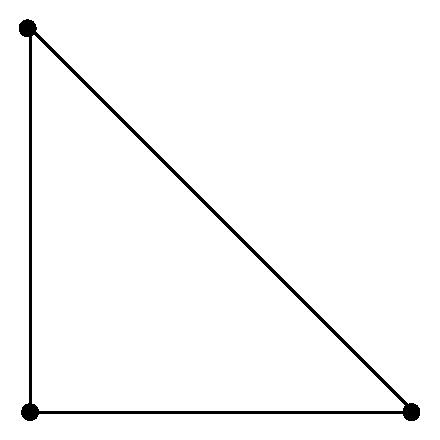
\includegraphics[width=5cm,angle=0]{getfemlist_triangle_P1.eps} & 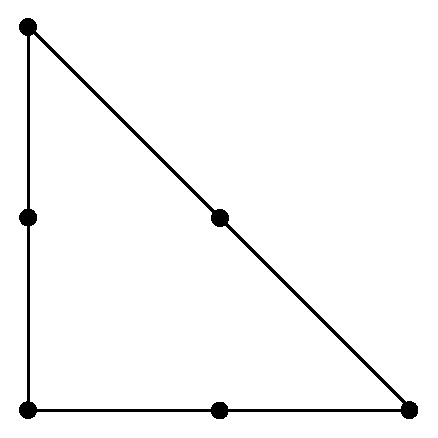
\includegraphics[width=5cm,angle=0]{getfemlist_triangle_P2.eps} \\
    $P_1$ element, 3 d.o.f., $C^0$ & $P_2$ element, 6 d.o.f., $C^0$ \\ \\
    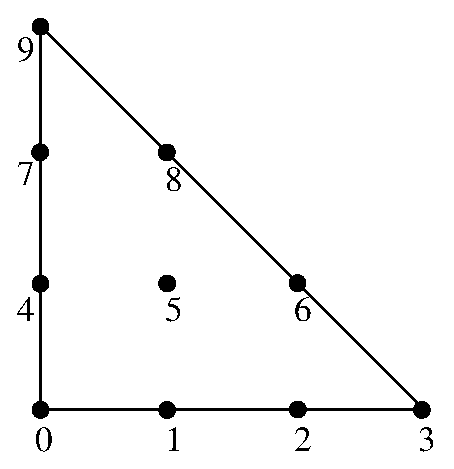
\includegraphics[width=5cm,angle=0]{getfemlist_triangle_P3.eps} & 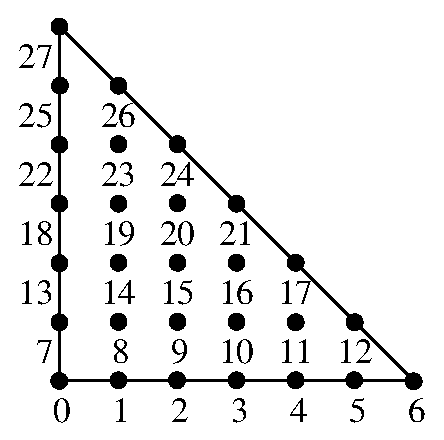
\includegraphics[width=5cm,angle=0]{getfemlist_triangle_P6.eps} \\
    $P_3$ element, 10 d.o.f., $C^0$ & $P_6$ element, 28 d.o.f., $C^0$
  \end{tabular} \end{center}
  \caption{ \it Examples of classical $P_K$ Lagrange elements on a triangle.} \label{fig:trianglepk}
\end{figure}

The number of degree of freedom for a classical ``$P_K$'' Lagrange element of dimension $P$ and degree $K$ is $\Frac{(P+K)!}{P!K!}$. For instance, in dimension 2 ($P = 2$), this value is $\Frac{(P+1) (P+2)}{2}$, in dimension 3 ($P = 3$), this value is $\Frac{(P+1) (P+2) (P+3)}{6}$ ...

\begin{figure}[H]
  \begin{center}
    \begin{tabular}{m{7cm}m{7cm}}
      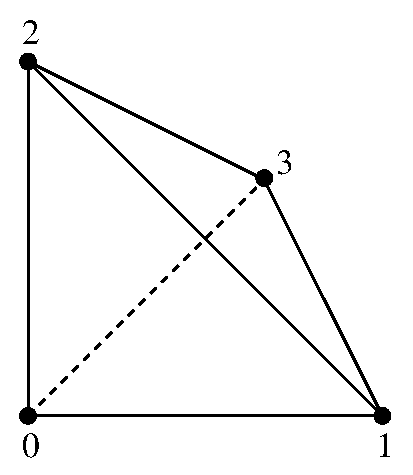
\includegraphics[width=5cm,angle=0]{getfemlist_tetrahedron_P1.eps} & 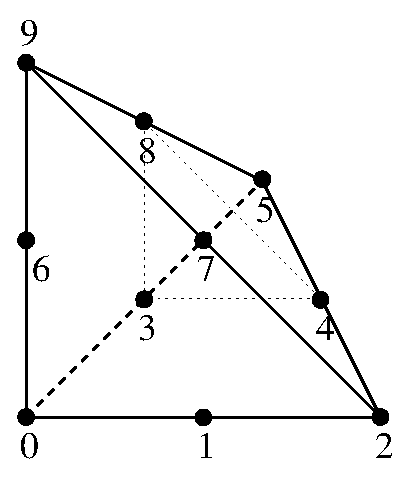
\includegraphics[width=5cm,angle=0]{getfemlist_tetrahedron_P2.eps} \\
      $P_1$ element, 4 d.o.f., $C^0$, & $P_2$ element, 10 d.o.f., $C^0$
    \end{tabular}
     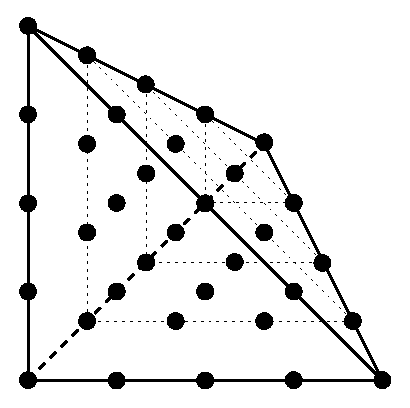
\includegraphics[width=5cm,angle=0]{getfemlist_tetrahedron_P4.eps} \\
     $P_4$ element, 35 d.o.f., $C^0$
  \end{center}
  \caption{ \it Examples of classical $P_K$ Lagrange elements on a tetrahedron.} \label{fig:tetrahedronpk}
\end{figure}

The particular way selected in {\sc Getfem++} to numerate the nodes are also shown in figures \ref{fig:segmentpk}, \ref{fig:trianglepk} and \ref{fig:tetrahedronpk}. Using another numeration, let 
$$ i_0, i_1, ... i_P, $$
be somme indexes such that
$$ 0 \leq i_0, i_1, ... i_P \leq K, \ \mbox{ and } \ \sum_{n = 0}^{P} i_n = K.$$
Then, the coordinate of a node can be computed as
$$ a_{i_0, i_1, ... i_P} = \sum_{n = 0}^{P} \Frac{i_n}{K}S_n, \ \ \mbox{ for } K \neq 0, $$
where $S_0, S_1, ... S_N$ are the vertexes of the simplex (for $K = 0$ the particular choice $a_{0, 0, ... 0} = \ds \sum_{n = 0}^{P} \Frac{1}{P+1}S_n$ has been chosen).
Then each base function, corresponding of each node $a_{i_0, i_1, ... i_P}$ is defined as
$$ \phi_{i_0, i_1, ... i_P} = \prod_{n = 0}^{P} \prod_{j=0}^{i_n-1} \left(\Frac{K \lambda_n - j}{j+1}\right).$$
where $\lambda_n$ are the barycentric coordinates, i.e. the polynomials of degree 1 whose value is $1$ on the vertex $S_n$ and whose value is $0$ on other vertices. On the reference element, one has
$$ \lambda_n = x_n, \ \ 0 \leq n < P, $$
$$ \lambda_P = 1 - x_0 - x_1 - ... - x_{P-1}. $$

When between two elements of the same degrees (even with different dimensions), the d.o.f. of a common face are linked, the element is of class $C^0$. This means that the global polynomial is continuous. If you try to link elements of different degrees, you will get some trouble with the unlinked d.o.f. This is not automatically supported by {\sc Getfem++}, so you will have to support it (add constraints on these d.o.f.).\\

For some applications (computation of a gradient for instance) one does not want the d.o.f. of a common face to be linked. This is why there are two versions of the classical ``$P_K$'' Lagrange element.\\[1cm]

\begin{center}
\begin{tabular}{|m{16.109cm}|} \hline
{\bf Classical ``$P_K$'' Lagrange element}\\
{\tt "FEM\_PK(P, K)"} 
\end{tabular} \\ \vspace{-1pt} 
\begin{tabular}{|m{2cm}|m{2cm}|m{2.5cm}|m{1.5cm}|m{1.5cm}|m{2cm}|m{2cm}|} \hline 
Degree & dimension & d.o.f. number & class & vectorial & \mbox{$\tau$-equivalent} & Polynomial \\ \hline
\small $K$, \mbox{$0 \leq K \leq 255$} & \small $P$, \mbox{$\ 1 \leq P \leq 255$} & $\Frac{(K+P)!}{K! P!}$ & $C^0$ & No \mbox{($Q = 1$)} & Yes \mbox{($\tilde{M} = Id$)} & Yes \\ \hline
\end{tabular}
\end{center}
\begin{center}
\begin{tabular}{|m{16.109cm}|} \hline 
{\bf Discontinuous ``$P_K$'' Lagrange element}\\
{\tt "FEM\_PK\_DISCONTINUOUS(P, K)"} 
\end{tabular} \\ \vspace{-1pt} 
\begin{tabular}{|m{2cm}|m{2cm}|m{2.5cm}|m{1.5cm}|m{1.5cm}|m{2cm}|m{2cm}|} \hline 
Degree & dimension & d.o.f. number & class & vectorial & \mbox{$\tau$-equivalent} & Polynomial \\ \hline
\small $K$, \mbox{$0 \leq K \leq 255$} & \small $P$, \mbox{$\ 1 \leq P \leq 255$} & $\Frac{(K+P)!}{K! P!}$ & discon-tinuous & No \mbox{($Q = 1$)} & Yes \mbox{($\tilde{M} = Id$)} & Yes \\ \hline
\end{tabular}
\end{center}$\ $\\[3cm]

Even thought Lagrange elements are defined for arbitrary degrees, to choose a hight degree can be problematic for a large number of applications due to the ``noisy'' caracteristic of the lagrange basis. Those element are recommended for the basic interpolation but for p.d.e. applications elements with hierarchical basis are preferable (see the corresponding section).

\subsection{Classical Lagrange elements on other geometries}

Classical Lagrange elements on parallelepipeds or prisms are obtained as tensorial product of Lagrange elements on simplices. When two element are defined, one on a dimension $P_1$ and the other in dimension $P_2$, one obtains the base functions of the tensorial product (on the reference element) as
$$ \hat{\phi}_{ij}(x,y) = \hat{\phi}^1_i(x) \hat{\phi}^2_j(y), \ \ x \in \Reel^{P_1}, y \in  \Reel^{P_2}, $$
where $\hat{\phi}^1_i$ and $\hat{\phi}^2_i$ are respectively the base functions of the first and second element.


\begin{figure}[H]
  \begin{center} \begin{tabular}{m{7cm}m{7cm}}
    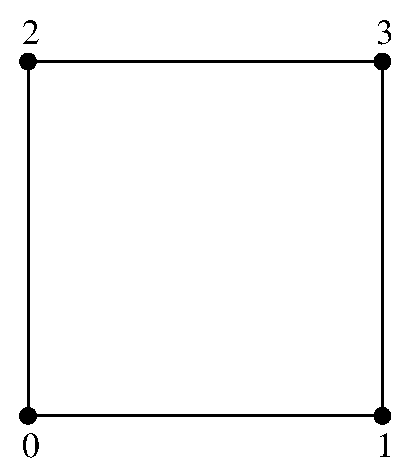
\includegraphics[width=5cm,angle=0]{getfemlist_quad_Q1.eps} & 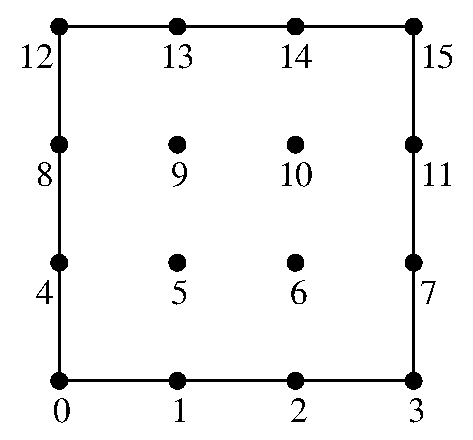
\includegraphics[width=5cm,angle=0]{getfemlist_quad_Q3.eps} \\
    $Q_1$ element, 4 d.o.f., $C^0$ & $Q_3$ element, 16 d.o.f., $C^0$ \\
  \end{tabular} \end{center}
  \caption{ \it Examples of classical Lagrange elements in dimension 2} \label{fig:prodpkdeux}
\end{figure}

The $Q_K$ element on a parallelepiped of dimension $P$ is obtained as the tensorial product of $P$ classical $P_K$ element on the segment. Examples in dimension $2$ are shown in figure \ref{fig:prodpkdeux} and in dimension $3$ in figure \ref{fig:prodpktrois}. \\

A prism in dimension $P > 1$ is the direct product of a simplex of dimension $P-1$ with a segment. The $P_K \otimes P_K$ element on this prism is the tensorial product of the classical $P_K$ element on a simplex of dimension $P-1$ with the classical $P_K$ element on a segment. For $P=2$ this coincide with a parallelepiped. Examples in dimension $3$ are shown in figure \ref{fig:prodpktrois}. This is also possible not to have the same degree on each dimension. An example is shown on figure \ref{fig:prism_P2_p1}. 

\begin{figure}[H]
  \begin{center} \begin{tabular}{m{7cm}m{7cm}}
    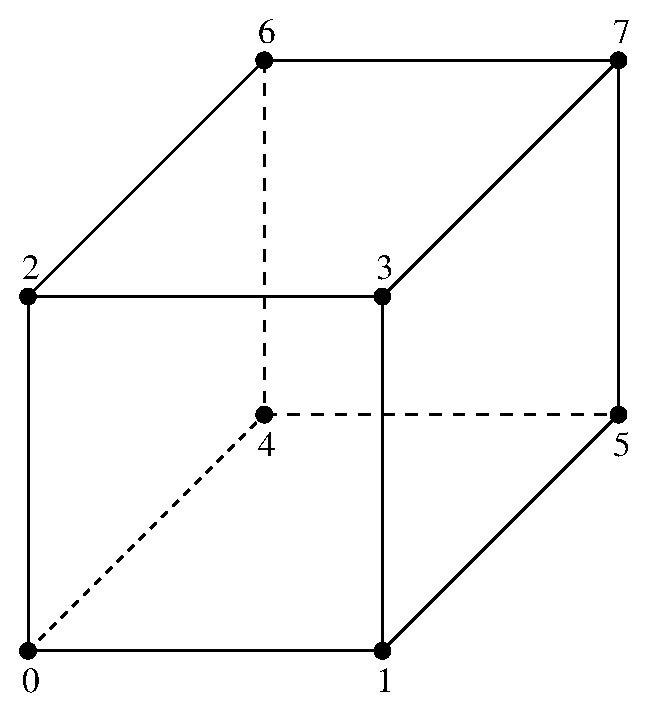
\includegraphics[width=5cm,angle=0]{getfemlist_cube_Q1.eps} & 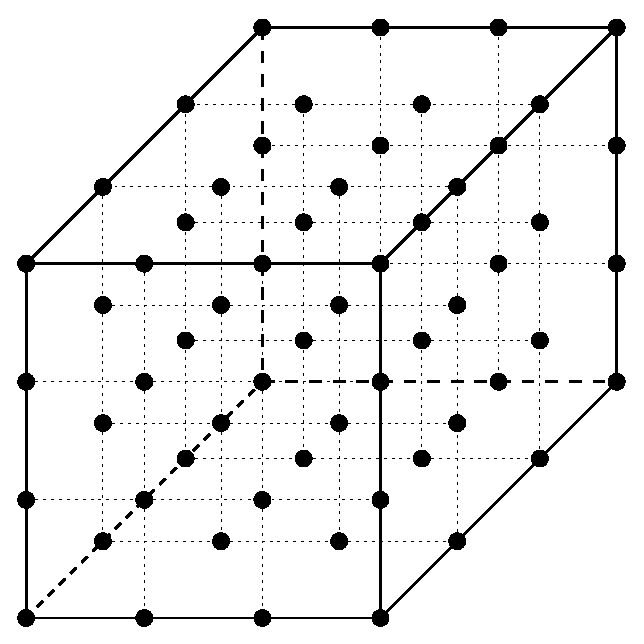
\includegraphics[width=5cm,angle=0]{getfemlist_cube_Q3.eps} \\
    $Q_1$ element, 8 d.o.f., $C^0$ & $Q_3$ element, 64 d.o.f., $C^0$ \\
    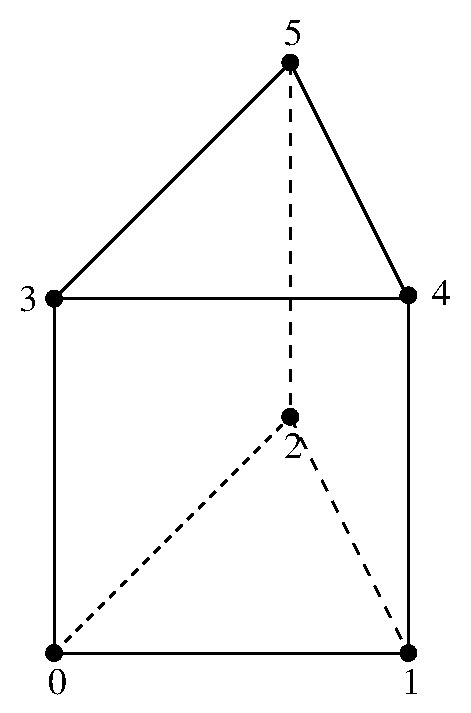
\includegraphics[width=3.5cm,angle=0]{getfemlist_prism_P1.eps} & 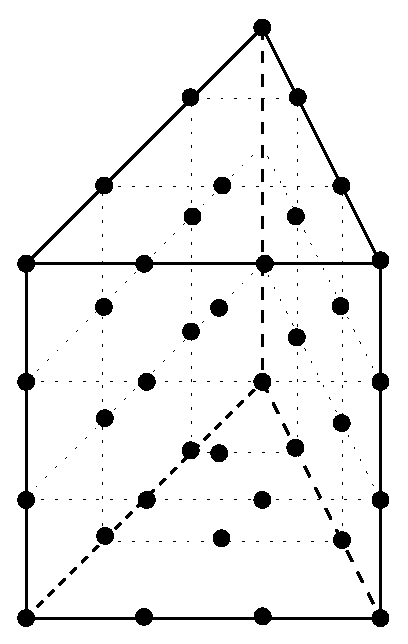
\includegraphics[width=3cm,angle=0]{getfemlist_prism_P3.eps} \\
    $P_1 \otimes P_1$ element, 6 d.o.f., $C^0$ & $P_3 \otimes P_3$ element, 40 d.o.f., $C^0$ \\
  \end{tabular} \end{center}
  \caption{ \it Examples of classical Lagrange elements in dimension 3} \label{fig:prodpktrois}
\end{figure}
\begin{figure}[H]
  \begin{center}
    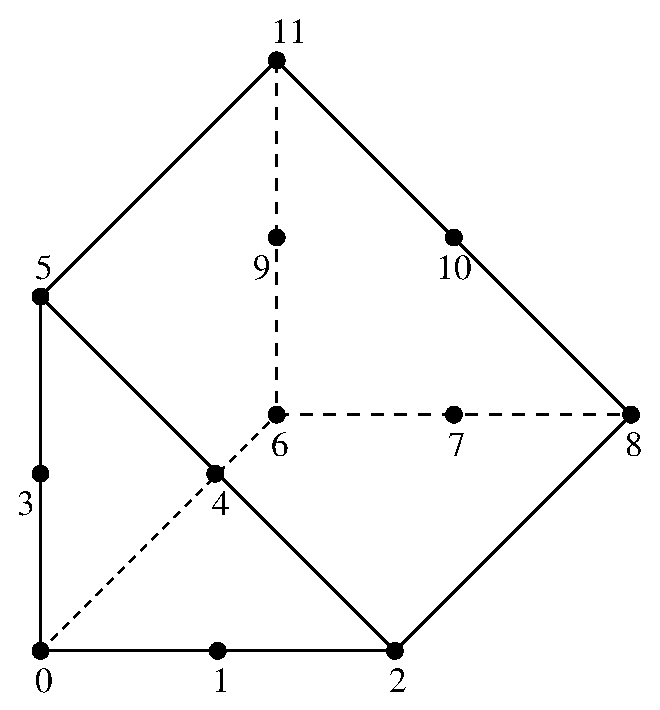
\includegraphics[width=3.5cm,angle=0]{getfemlist_prism_P2_P1.eps}
  \end{center}
  \caption{ \it $P_2 \otimes P_1$ Lagrange element on a prism, 12 d.o.f., $C^0$} 
  \label{fig:prism_P2_p1}
\end{figure}


\begin{center}
\begin{tabular}{|m{16.109cm}|} \hline 
{\bf $Q_K$ Lagrange element on parallelepipeds}\\
{\tt "FEM\_QK(P, K)"} 
\end{tabular} \\ \vspace{-1pt} 
\begin{tabular}{|m{2cm}|m{2cm}|m{2.5cm}|m{1.5cm}|m{1.5cm}|m{2cm}|m{2cm}|} \hline 
Degree & dimension & d.o.f. number & class & vectorial & \mbox{$\tau$-equivalent} & Polynomial \\ \hline
\small $KP$, \mbox{$0 \leq K \leq 255$} & \small $P$, \mbox{$\ 2 \leq P \leq 255$} & $(K+1)^P$ & $C^0$ & No \mbox{($Q = 1$)} & Yes \mbox{($\tilde{M} = Id$)}  & Yes \\ \hline
\end{tabular}
\end{center}

\begin{center}
\begin{tabular}{|m{16.109cm}|} \hline 
{\bf $P_K \otimes P_K$ Lagrange element on prisms}\\
{\tt "FEM\_PK\_PRISM(P, K)"} 
\end{tabular} \\ \vspace{-1pt} 
\begin{tabular}{|m{2cm}|m{2cm}|m{2.5cm}|m{1.5cm}|m{1.5cm}|m{2cm}|m{2cm}|} \hline 
Degree & dimension & d.o.f. number & class & vectorial & \mbox{$\tau$-equivalent} & Polynomial\\ \hline
\small $2K$, \mbox{$0 \leq K \leq 255$} & \small $P$, \mbox{$\ 2 \leq P \leq 255$} & \mbox{$(K+1)$} \mbox{$\times \Frac{(K+P-1)!}{K! (P-1)!}$} & $C^0$ & No \mbox{($Q = 1$)} & Yes \mbox{($\tilde{M} = Id$)}  & Yes\\ \hline
\end{tabular}
\end{center}

\begin{center}
\begin{tabular}{|m{16.109cm}|} \hline 
{\bf $P_{K_1} \otimes P_{K_2}$ Lagrange element on prisms}\\
{\tt "FEM\_PRODUCT(FEM\_PK(P-1, K$_1$), FEM\_PK(1, K$_2$))"} 
\end{tabular} \\ \vspace{-1pt} 
\begin{tabular}{|m{2cm}|m{2cm}|m{2.5cm}|m{1.5cm}|m{1.5cm}|m{2cm}|m{2cm}|} \hline 
Degree & dimension & d.o.f. number & class & vectorial & \mbox{$\tau$-equivalent} & Polynomial\\ \hline
\small \mbox{$K_1+K_2$}, \tiny \mbox{$0 \leq K_1,K_2 \leq 255$} & \small $P$, \mbox{$\ 2 \leq P \leq 255$} & \mbox{$(K_2+1)$} \mbox{$\times \Frac{(K_1+P-1)!}{K_1! (P-1)!}$} & $C^0$ & No \mbox{($Q = 1$)} & Yes \mbox{($\tilde{M} = Id$)}  & Yes\\ \hline
\end{tabular}
\end{center}

\begin{figure}[H]
  \begin{center}
    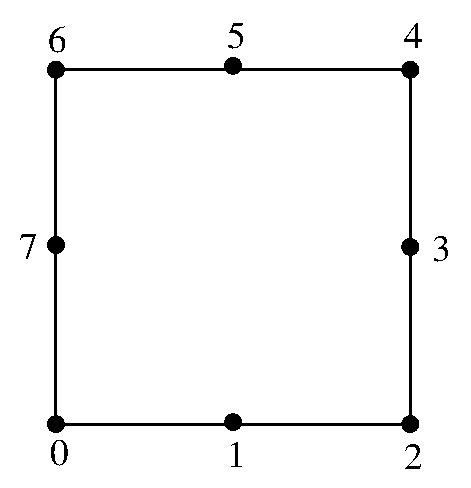
\includegraphics[width=5cm,angle=0]{getfemlist_quad8.eps} \\
    Incomplete $Q_2$ element, 8 d.o.f., $C^0$  \\
  \end{center}
\end{figure}

\begin{center}
\begin{tabular}{|m{16.109cm}|} \hline 
{\bf Incomplete $Q_2$ Lagrange element on quadrilateral (Quad 8 serendipity element)}\\
{\tt "FEM\_INCOMPLETE\_Q2"} 
\end{tabular} \\ \vspace{-1pt} 
\begin{tabular}{|m{2cm}|m{2cm}|m{2.5cm}|m{1.5cm}|m{1.5cm}|m{2cm}|m{2cm}|} \hline 
Degree & dimension & d.o.f. number & class & vectorial & \mbox{$\tau$-equivalent} & Polynomial \\ \hline
\small $3$ & 2 & 8 & $C^0$ & No \mbox{($Q = 1$)} & Yes \mbox{($\tilde{M} = Id$)}  & Yes \\ \hline
\end{tabular}
\end{center}

\subsection{Elements with hierarchical basis}

The idea behind hierarchical basis is the desciption of the solution at different level : a rought level, a more refined level ... In the same discretisation some degrees of freedom represent the rought description, some other the more rafined and so on. This correspond to imbricated spaces of discretisation. The hierarchical basis contains a basis of each of these spaces (this is not the case in classical Lagrange elements when the mesh is refined).\\[0.5cm]
Among the advantages, the condition number of  rigidity matrices can be greatly improved, it allows local raffinement and a resolution with a multigrid approach.


\subsubsection{Hiercarchical elements with respect to the degree}

\begin{figure}[H]
  \begin{center}
    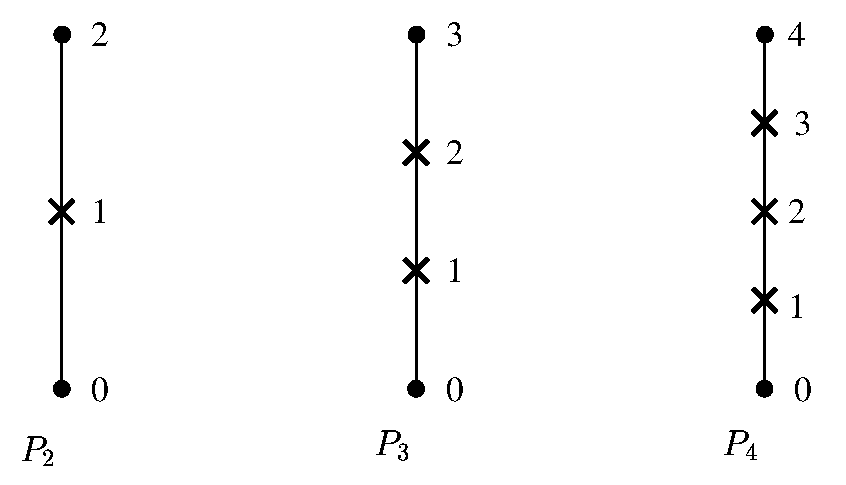
\includegraphics[width=5cm,angle=0]{getfemlist_segment_hier.eps}
  \end{center}
  \caption{ \it $P_K$ Hierarchical element on a segment, $C^0$} 
  \label{fig:seg_hier}
\end{figure}


\begin{center}
\begin{tabular}{|m{16.109cm}|} \hline 
{\bf $P_{K}$ Classical Lagrange element on simplices but with a hierarchical basis with respect to the degree}\\
{\tt "FEM\_PK\_HIERARCHICAL(P,K)"} 
\end{tabular} \\ \vspace{-1pt} 
\begin{tabular}{|m{2cm}|m{2cm}|m{2.5cm}|m{1.5cm}|m{1.5cm}|m{2cm}|m{2cm}|} \hline 
Degree & dimension & d.o.f. number & class & vectorial & \mbox{$\tau$-equivalent} & Polynomial\\ \hline
\small \mbox{$K$}, \small \mbox{$0 \leq K\leq 255$} & \small $P$, \mbox{$\ 1 \leq P \leq 255$} & \mbox{$\Frac{(K_1+P)!}{K_1! P!}$} & $C^0$ & No \mbox{($Q = 1$)} & Yes \mbox{($\tilde{M} = Id$)}  & Yes\\ \hline
\end{tabular}
\end{center}

\begin{center}
\begin{tabular}{|m{16.109cm}|} \hline 
{\bf $Q_{K}$ Classical Lagrange element on parallelepipeds but with a hierarchical basis with respect to the degree}\\
{\tt "FEM\_QK\_HIERARCHICAL(P,K)"} 
\end{tabular} \\ \vspace{-1pt} 
\begin{tabular}{|m{2cm}|m{2cm}|m{2.5cm}|m{1.5cm}|m{1.5cm}|m{2cm}|m{2cm}|} \hline 
Degree & dimension & d.o.f. number & class & vectorial & \mbox{$\tau$-equivalent} & Polynomial\\ \hline
\small \mbox{$K$}, \small \mbox{$0 \leq K\leq 255$} & \small $P$, \mbox{$\ 2 \leq P \leq 255$} & \mbox{$(K+1)^P$} & $C^0$ & No \mbox{($Q = 1$)} & Yes \mbox{($\tilde{M} = Id$)}  & Yes\\ \hline
\end{tabular}
\end{center}

\begin{center}
\begin{tabular}{|m{16.109cm}|} \hline 
{\bf $P_{K}$ Classical Lagrange element on prisms but with a hierarchical basis with respect to the degree}\\
{\tt "FEM\_PK\_PRISM\_HIERARCHICAL(P,K)"} 
\end{tabular} \\ \vspace{-1pt} 
\begin{tabular}{|m{2cm}|m{2cm}|m{2.5cm}|m{1.5cm}|m{1.5cm}|m{2cm}|m{2cm}|} \hline 
Degree & dimension & d.o.f. number & class & vectorial & \mbox{$\tau$-equivalent} & Polynomial\\ \hline
\small \mbox{$K$}, \small \mbox{$0 \leq K\leq 255$} & \small $P$, \mbox{$\ 2 \leq P \leq 255$} & \mbox{$(K+1)$} \mbox{$\times \Frac{(K+P-1)!}{K! (P-1)!}$} & $C^0$ & No \mbox{($Q = 1$)} & Yes \mbox{($\tilde{M} = Id$)}  & Yes\\ \hline
\end{tabular}
\end{center}

some particular choices : $P_4$ will be build with the basis of the $P_1$, the additional basis of the $P_2$ then the additionnal basis of the $P_4$.

$P_6$ will be build  with the basis of the $P_1$, the additional basis of the $P_2$ then the additionnal basis of the $P_6$ (not with the basis of the $P_1$, 
the additional basis of the $P_3$ then the additionnal basis of the $P_6$, this is possible to build the latter with {\tt "FEM\_GEN\_HIERARCHICAL(a,b)})

\subsubsection{Composite elements}

The principal interest of the composite elements is to build hierarchical elements. But this tool can also be used to build piecewise polynomial elements.

\begin{figure}[H]
  \begin{center}
    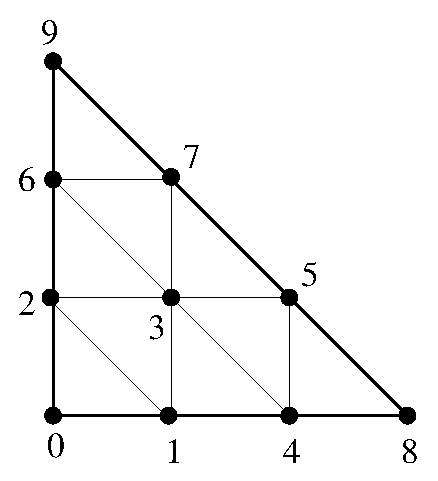
\includegraphics[width=5cm,angle=0]{getfemlist_triangle_P1comp.eps}
  \end{center}
  \caption{ \it composite element {\tt "FEM\_STRUCTURED\_COMPOSITE(FEM\_PK(2,1), 3)"}} 
  \label{fig:triangle_comp}
\end{figure}

\begin{center}
\begin{tabular}{|m{16.109cm}|} \hline 
{\bf composition of a finite element method on a element with {\tt S} subdivisions}\\
{\tt "FEM\_STRUCTURED\_COMPOSITE(FEM1, S)"} 
\end{tabular} \\ \vspace{-1pt} 
\begin{tabular}{|m{2cm}|m{2cm}|m{2.5cm}|m{1.5cm}|m{1.5cm}|m{2cm}|m{2cm}|} \hline 
Degree & dimension & d.o.f. number & class & vectorial & \mbox{$\tau$-equivalent} & Polynomial\\ \hline
\small degree of FEM1 & \small dimension of FEM1 & variable & variable & No \mbox{($Q = 1$)} & If {\tt FEM1} is  & piecewise\\ \hline
\end{tabular}
\end{center}

It is important to use a corresponding composite integration method.

\subsubsection{Hierarchical composite elements}

\begin{figure}[H]
  \begin{center}
    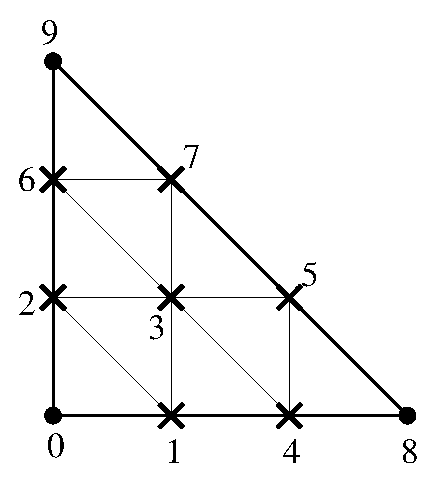
\includegraphics[width=5cm,angle=0]{getfemlist_triangle_P1comp_hier.eps}
  \end{center}
  \caption{ \it hierarchical composite element {\tt "FEM\_PK\_HIERARCHICAL\_COMPOSITE(2,1,3)"}} 
  \label{fig:triangle_comp}
\end{figure}

\begin{center}
\begin{tabular}{|m{16.109cm}|} \hline 
{\bf hierarchical composition of a $P_K$ finite element method on a simplex with {\tt S} subdivisions}\\
{\tt "FEM\_PK\_HIERARCHICAL\_COMPOSITE(P,K,S)"} 
\end{tabular} \\ \vspace{-1pt} 
\begin{tabular}{|m{2cm}|m{2cm}|m{2.5cm}|m{1.5cm}|m{1.5cm}|m{2cm}|m{2cm}|} \hline 
Degree & dimension & d.o.f. number & class & vectorial & \mbox{$\tau$-equivalent} & Polynomial\\ \hline
\small K & \small P & \mbox{$\Frac{(SK+P)!}{(SK)! P!}$} & variable & No \mbox{($Q = 1$)} & If {\tt FEM1} is  & piecewise\\ \hline
\end{tabular}
\end{center}

\begin{center}
\begin{tabular}{|m{16.109cm}|} \hline 
{\bf hierarchical composition of a hierarchical $P_K$ finite element method on a simplex with {\tt S} subdivisions}\\
{\tt "FEM\_PK\_FULL\_HIERARCHICAL\_COMPOSITE(P,K,S)"} 
\end{tabular} \\ \vspace{-1pt} 
\begin{tabular}{|m{2cm}|m{2cm}|m{2.5cm}|m{1.5cm}|m{1.5cm}|m{2cm}|m{2cm}|} \hline 
Degree & dimension & d.o.f. number & class & vectorial & \mbox{$\tau$-equivalent} & Polynomial\\ \hline
\small K & \small P & \mbox{$\Frac{(SK+P)!}{(SK)! P!}$} & variable & No \mbox{($Q = 1$)} & If {\tt FEM1} is  & piecewise\\ \hline
\end{tabular}
\end{center}

Other constructions are possible thanks to {\tt "FEM\_GEN\_HIERARCHICAL(FEM1, FEM2)"} and \\ {\tt "FEM\_STRUCTURED\_COMPOSITE(FEM1, S)"}

It is important to use a corresponding composite integration method.

\subsection{Specific elements in dimension 1}

\subsubsection{GaussLobatto element}

The 1D GaussLobatto $P_K$ element is similar to the classical $P_K$ fem on the segment, but
the nodes are given by the Gauss-Lobatto-Legendre quadrature rule of
order $2K-1$. This FEM is known to lead to better conditioned linear
systems, and can be used with the correspounding quadrature to perform
mass-lumping (on segments or parallelepipeds).

The polynomials coefficients have been pre-computed with Maple (they require the inversion of an ill-conditionned system), hence they are only available for the following values \\ of $K$: $1, 2, 3, 4, 5, 6, 7, 8, 9, 10, 11, 12, 13, 14, 16, 24, 32$. Note that for $K=1$ and $K=2$, this is the classical $P1$ and $P2$ fem.

\begin{center}
\begin{tabular}{|m{16.11cm}|} \hline 
{\bf GaussLobatto $P_K$ element on the segment}\\
{\tt "FEM\_PK\_GAUSSLOBATTO1D(K)"}
\end{tabular} \\ \vspace{-1pt} 
\begin{tabular}{|m{2cm}|m{2cm}|m{2.5cm}|m{1.2cm}|m{2cm}|m{2cm}|m{1.8cm}|} \hline 
Degree & dimension & d.o.f. number & class & vectorial & \mbox{$\tau$-equivalent} & Polynomial\\ \hline
$K$ & $1$ & $K+1$ & $C^0$ & No \mbox{($Q = 1$)} & Yes & Yes\\ \hline
\end{tabular}
\end{center}

\subsubsection{Hermite element}

\begin{figure}[H]
  \begin{center}
    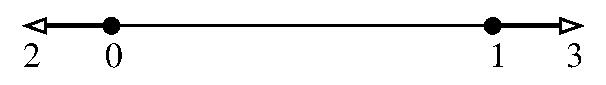
\includegraphics[width=5cm,angle=0]{getfemlist_segment_hermite.eps}
  \end{center}
  \caption{ \it $P_3$ Hermite element on a segment, 4 d.o.f., $C^1$} 
  \label{fig:segment_hermite}
\end{figure}

Base functions on the reference element
\begin{eqnarray*}
 \hat{\varphi}_0 = (2x+1)(x-1)^2,&&\ \ \ \hat{\varphi}_1 = x^2(3-2x), \\
 \hat{\varphi}_2 = x(x-1)^2,&& \ \ \ \hat{\varphi}_3 = x^2(x - 1). 
\end{eqnarray*}

This element is close to be \mbox{$\tau$-equivalent} but it is not. On the real element the value of the gradient on vertices will be multiplied by the gradient of the geometric transformation. The matrix $\tilde{M}$ is not equal to identity but is still diagonal.

\begin{center}
\begin{tabular}{|m{16.11cm}|} \hline 
{\bf Hermite element on the segment}\\
{\tt "FEM\_HERMITE(1)"}
\end{tabular} \\ \vspace{-1pt} 
\begin{tabular}{|m{2cm}|m{2cm}|m{2.5cm}|m{1.2cm}|m{2cm}|m{2cm}|m{1.8cm}|} \hline 
Degree & dimension & d.o.f. number & class & vectorial & \mbox{$\tau$-equivalent} & Polynomial\\ \hline
$3$ & $1$ & $4$ & $C^1$ & No \mbox{($Q = 1$)} & No & Yes\\ \hline
\end{tabular}
\end{center}

\subsubsection{Lagrange element with an additional bubble function}

\begin{figure}[H]
  \begin{center}
    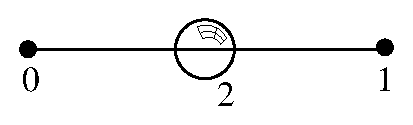
\includegraphics[width=5cm,angle=0]{getfemlist_segment_bubble.eps}
  \end{center}
  \caption{ \it $P_1$ Lagrange element on a segment with additional internal bubble function, 3 d.o.f., $C^0$} 
  \label{fig:segment_bubble}
\end{figure}

\begin{center}
\begin{tabular}{|m{16.11cm}|} \hline 
{ \bf Lagrange $P_1$ element with an additional internal bubble function}\\
{\tt "FEM\_PK\_WITH\_CUBIC\_BUBBLE(1, 1)"} 
\end{tabular} \\ \vspace{-1pt} 
\begin{tabular}{|m{2cm}|m{2cm}|m{2.5cm}|m{1.2cm}|m{2cm}|m{2cm}|m{1.8cm}|} \hline 
Degree & dimension & d.o.f. number & class & vectorial & \mbox{$\tau$-equivalent} & Polynomial\\ \hline
$2$ & $1$ & $3$ & $C^0$ & No \mbox{($Q = 1$)} & Yes & Yes\\ \hline
\end{tabular}
\end{center}

\subsection{Specific elements in dimension 2}
\subsubsection{Elements with additional bubble functions}

\begin{figure}[H]
  \begin{center}
    \begin{tabular}{m{7cm}m{7cm}}
      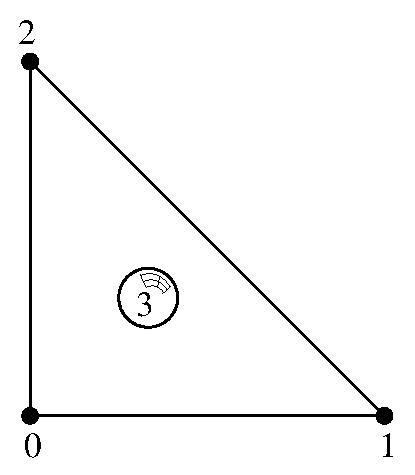
\includegraphics[width=5cm,angle=0]{getfemlist_triangle_P1_bubble.eps} & 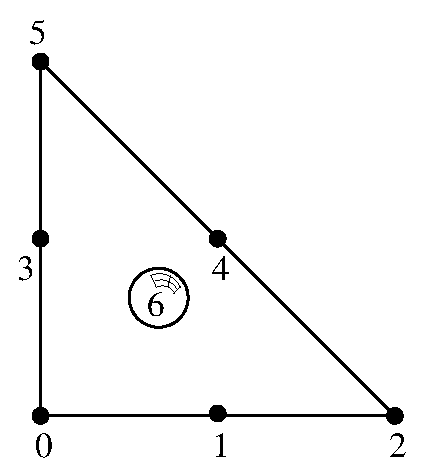
\includegraphics[width=5cm,angle=0]{getfemlist_triangle_P2_bubble.eps}  \\
      $P_1$ with additional bubble function, 4 d.o.f., $C^0$ & $P_2$ with additional bubble function, 7 d.o.f., $C^0$
    \end{tabular}
  \end{center}
  \caption{ \it Lagrange element on a triangle with additional internal bubble function} 
  \label{fig:triangle_p1_bubble}
\end{figure}

\begin{center}
\begin{tabular}{|m{16.11cm}|} \hline 
{ \bf Lagrange $P_1$ or $P_2$ element with an additional internal bubble function}\\
{\tt "FEM\_PK\_WITH\_CUBIC\_BUBBLE(2, K)"} 
\end{tabular} \\ \vspace{-1pt} 
\begin{tabular}{|m{2cm}|m{2cm}|m{2.5cm}|m{1.2cm}|m{2cm}|m{2cm}|m{1.8cm}|} \hline 
Degree & dimension & d.o.f. number & class & vectorial & \mbox{$\tau$-equivalent} & Polynomial\\ \hline
$3$ & $2$ & $4$ or $7$ & $C^0$ & No \mbox{($Q = 1$)} & Yes & Yes\\ \hline
\end{tabular}
\end{center}

\begin{figure}[H]
  \begin{center}
    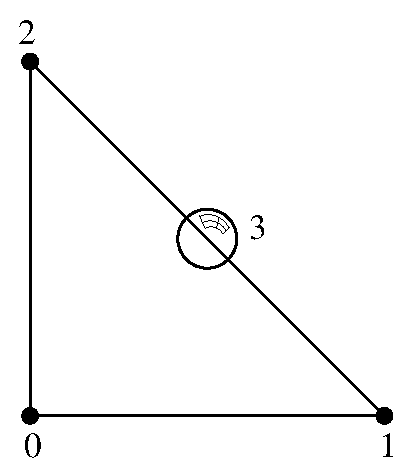
\includegraphics[width=5cm,angle=0]{getfemlist_triangle_P1_bubble_face.eps}
  \end{center}
  \caption{ \it $P_1$ Lagrange element on a triangle with additional bubble function on face 0, 4 d.o.f., $C^0$} 
  \label{fig:triangle_p1_bubble_face}
\end{figure}

\begin{center}
\begin{tabular}{|m{16.11cm}|} \hline 
{ \bf Lagrange $P_1$ element with an additional bubble function on face 0}\\
{\tt "FEM\_P1\_BUBBLE\_FACE(2)"} 
\end{tabular} \\ \vspace{-1pt} 
\begin{tabular}{|m{2cm}|m{2cm}|m{2.5cm}|m{1.2cm}|m{2cm}|m{2cm}|m{1.8cm}|} \hline 
Degree & dimension & d.o.f. number & class & vectorial & \mbox{$\tau$-equivalent} & Polynomial\\ \hline
$2$ & $2$ & $4$ & $C^0$ & No \mbox{($Q = 1$)} & Yes & Yes\\ \hline
\end{tabular}
\end{center}

\begin{figure}[H]
  \begin{center}
    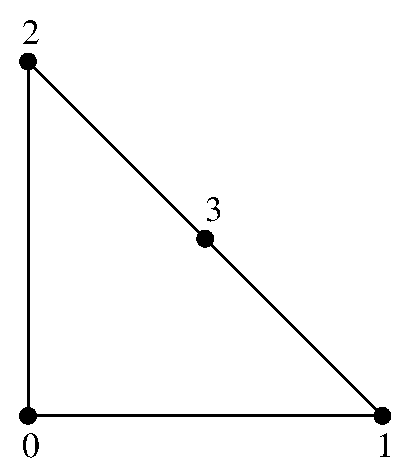
\includegraphics[width=5cm,angle=0]{getfemlist_triangle_P1_with_P2_face.eps}
  \end{center}
  \caption{ \it $P_1$ Lagrange element on a triangle with additional d.o.f on face 0, 4 d.o.f., $C^0$} 
  \label{fig:triangle_p1_p2_face}
\end{figure}

\begin{center}
\begin{tabular}{|m{16.11cm}|} \hline 
{ \bf $P_1$ Lagrange element on a triangle with additional d.o.f on face 0}\\
{\tt "FEM\_P1\_BUBBLE\_FACE\_LAG"} 
\end{tabular} \\ \vspace{-1pt} 
\begin{tabular}{|m{2cm}|m{2cm}|m{2.5cm}|m{1.2cm}|m{2cm}|m{2cm}|m{1.8cm}|} \hline 
Degree & dimension & d.o.f. number & class & vectorial & \mbox{$\tau$-equivalent} & Polynomial\\ \hline
$2$ & $2$ & $4$ & $C^0$ & No \mbox{($Q = 1$)} & Yes & Yes\\ \hline
\end{tabular}
\end{center}

\subsubsection{Non-conforming $P_1$ element}


\begin{figure}[H]
  \begin{center}
    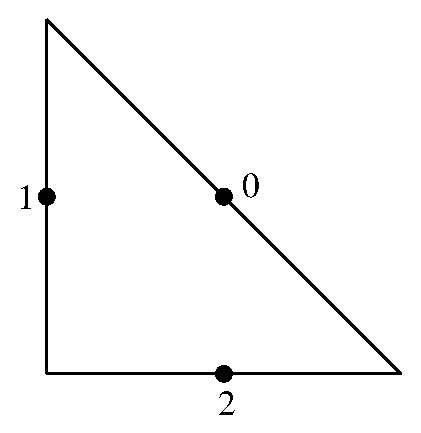
\includegraphics[width=5cm,angle=0]{getfemlist_triangle_P1_non_conforming.eps}
  \end{center}
  \caption{ \it $P_1$ non-conforming element on a triangle, 3 d.o.f., discontinuous} 
  \label{fig:triangle_non_conforming}
\end{figure}

\begin{center}
\begin{tabular}{|m{16.11cm}|} \hline 
{ \bf $P_1$ non-conforming element on a triangle}\\
{\tt "FEM\_P1\_NONCONFORMING"} 
\end{tabular} \\ \vspace{-1pt} 
\begin{tabular}{|m{2cm}|m{2cm}|m{2.5cm}|m{1.2cm}|m{2cm}|m{2cm}|m{1.8cm}|} \hline 
Degree & dimension & d.o.f. number & class & vectorial & \mbox{$\tau$-equivalent} & Polynomial\\ \hline
$1$ & $2$ & $3$ & discon-tinuous & No \mbox{($Q = 1$)} & Yes & Yes\\ \hline
\end{tabular}
\end{center}

\subsubsection{Hermite element}

\begin{figure}[H]
  \begin{center}
    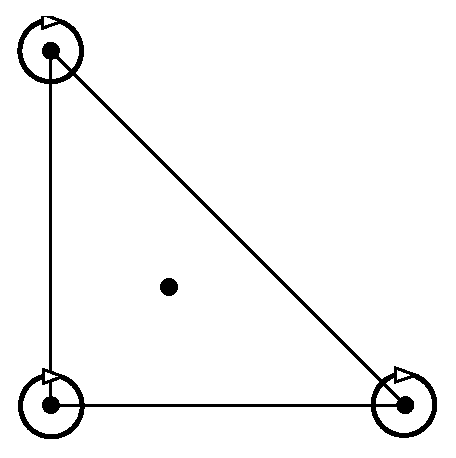
\includegraphics[width=6cm,angle=0]{getfemlist_triangle_hermite.eps}
  \end{center}
  \caption{ \it Hermite element on a triangle, $P_3$, 10 d.o.f., $C^0$ }
  \label{fig:triangle_hermite}
\end{figure}

Base functions on the reference element:
$$
  \begin{array}{ll}
 \hat{\varphi}_0 = (1-x-y)(1+x+y-2x^2-2y^2-11xy),~~ & (\hat{\varphi}_0(0,0) = 1), \\
 \hat{\varphi}_1 = -2x^3 + 7 x^2y + 7xy^2 + 3x^2 - 7xy, & (\hat{\varphi}_1(1,0) = 1), \\
 \hat{\varphi}_2 = 7x^2y + 7xy^2 - 2y^3+3y^2-7xy, & (\hat{\varphi}_2(0,1) = 1), \\
 \hat{\varphi}_3 = 27xy(1-x-y), & (\hat{\varphi}_3(1/3,1/3) = 1), \\
 \hat{\varphi}_4 = x(1-x-y)(1-x-2y), & (\partial_x\hat{\varphi}_4(0,0) = 1), \\
 \hat{\varphi}_5 = x^3-2x^2y-2xy^2-x^2+2xy, & (\partial_x\hat{\varphi}_5(1,0) = 1), \\
 \hat{\varphi}_6 = xy(x+2y-1), & (\partial_x\hat{\varphi}_6(0,1) = 1), \\
 \hat{\varphi}_7 = y(1-x-y)(1-2x-y), & (\partial_y\hat{\varphi}_7(0,0) = 1), \\
 \hat{\varphi}_8 = xy(y+2x-1), & (\partial_y\hat{\varphi}_8(1,0) = 1), \\
 \hat{\varphi}_9 = y^3-2x^2y-2xy^2-y^2+2xy, & (\partial_y\hat{\varphi}_9(0,1) = 1), \\
  
  \end{array}
$$
This element is not \mbox{$\tau$-equivalent} (The matrix $\tilde{M}$ is not equal to identity). On the real element linear combinaisons of $\hat{\varphi}_4$ and $\hat{\varphi}_7$ are used to match the gradient on the corresponding vertex. Idem for the two couples ($\hat{\varphi}_5$, $\hat{\varphi}_8$) and  ($\hat{\varphi}_6$, $\hat{\varphi}_9$) for the two other vertices.  

\begin{center}
\begin{tabular}{|m{16.11cm}|} \hline 
{ \bf Hermite element on a triangle}\\
"FEM\_HERMITE(2)"
\end{tabular} \\ \vspace{-1pt} 
\begin{tabular}{|m{2cm}|m{2cm}|m{2.5cm}|m{1.2cm}|m{2cm}|m{2cm}|m{1.8cm}|} \hline 
Degree & dimension & d.o.f. number & class & vectorial & \mbox{$\tau$-equivalent} & Polynomial\\ \hline
$3$ & $2$ & $10$ & $C^0$ & No \mbox{($Q = 1$)} & No & Yes\\ \hline
\end{tabular}
\end{center}

\subsubsection{Argyris element}

\begin{figure}[H]
  \begin{center}
    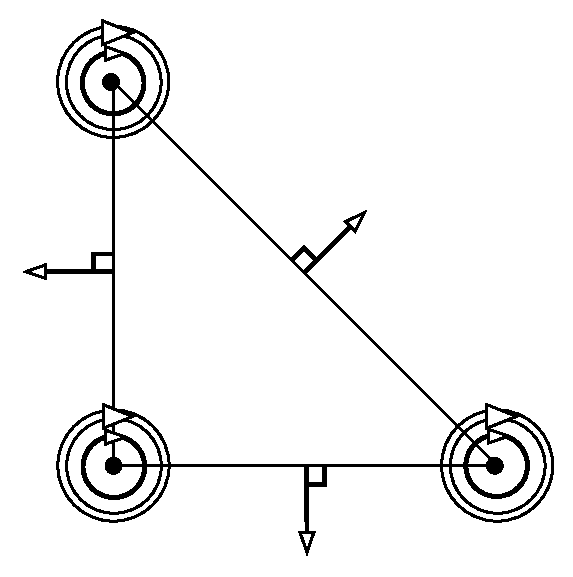
\includegraphics[width=6cm,angle=0]{getfemlist_argyris.eps}
  \end{center}
  \caption{ \it Argyris element, $P_5$, 21 d.o.f., $C^1$}
  \label{fig:argyris}
\end{figure}

The base functions on the reference element are:
$$ \begin{array}{ll}
\hat{\varphi}_{0}(x,y) = 1 - 10x^3 - 10y^3 + 15x^4 - 30x^2y^2 + 15y^4 - 6x^5 + 30x^3y^2 + 30x^2y^3 - 6y^5, & (\hat{\varphi}_0(0,0) = 1), \\
\hat{\varphi}_{1}(x,y) = 10x^3 - 15x^4 + 15x^2y^2 + 6x^5 - 15x^3y^2 - 15x^2y^3, & (\hat{\varphi}_1(1,0) = 1),\\
\hat{\varphi}_{2}(x,y) = 10y^3 + 15x^2y^2 - 15y^4 - 15x^3y^2 - 15x^2y^3 + 6y^5, & (\hat{\varphi}_2(0,1) = 1),\\
\hat{\varphi}_{3}(x,y) = x - 6x^3 - 11xy^2 + 8x^4 + 10x^2y^2 + 18xy^3 - 3x^5 + x^3y^2 - 10x^2y^3 - 8xy^4, & (\partial_x\hat{\varphi}_3(0,0) = 1),\\
\hat{\varphi}_{4}(x,y) = -4x^3 + 7x^4 - 3.5x^2y^2 - 3x^5 + 3.5x^3y^2 + 3.5x^2y^3, & (\partial_x\hat{\varphi}_4(1,0) = 1),\\
\hat{\varphi}_{5}(x,y) = -5xy^2 + 18.5x^2y^2 + 14xy^3 - 13.5x^3y^2 - 18.5x^2y^3 - 8xy^4, & (\partial_x\hat{\varphi}_5(0,1) = 1),\\
\hat{\varphi}_{6}(x,y) = y - 11x^2y - 6y^3 + 18x^3y + 10x^2y^2 + 8y^4 - 8x^4y - 10x^3y^2 + x^2y^3 - 3y^5, & (\partial_y\hat{\varphi}_6(0,0) = 1),\\
\hat{\varphi}_{7}(x,y) = -5x^2y + 14x^3y + 18.5x^2y^2 - 8x^4y - 18.5x^3y^2 - 13.5x^2y^3, & (\partial_y\hat{\varphi}_7(1,0) = 1),\\
\hat{\varphi}_{8}(x,y) = -4y^3 - 3.5x^2y^2 + 7y^4 + 3.5x^3y^2 + 3.5x^2y^3 - 3y^5, & (\partial_y\hat{\varphi}_8(0,0) = 1),\\
\hat{\varphi}_{9}(x,y) = 0.5x^2 - 1.5x^3 + 1.5x^4 - 1.5x^2y^2 - 0.5x^5 + 1.5x^3y^2 + x^2y^3, & (\partial^2_{xx}\hat{\varphi}_9(0,0) = 1),\\
\hat{\varphi}_{10}(x,y) = 0.5x^3 - x^4 + 0.25x^2y^2 + 0.5x^5 - 0.25x^3y^2 - 0.25x^2y^3, & (\partial^2_{xx}\hat{\varphi}_{10}(1,0) = 1),\\
\hat{\varphi}_{11}(x,y) = 1.25x^2y^2 - 1.25x^3y^2 - 0.75x^2y^3, & (\partial^2_{xx}\hat{\varphi}_{11}(0,1) = 1),\\
\hat{\varphi}_{12}(x,y) = xy - 4x^2y - 4xy^2 + 5x^3y + 10x^2y^2 + 5xy^3 - 2x^4y - 6x^3y^2 - 6x^2y^3 - 2xy^4, & (\partial^2_{xy}\hat{\varphi}_{12}(0,0) = 1),\\
\hat{\varphi}_{13}(x,y) = x^2y - 3x^3y - 3.5x^2y^2 + 2x^4y + 3.5x^3y^2 + 2.5x^2y^3, & (\partial^2_{xy}\hat{\varphi}_{13}(1,0) = 1),\\
\hat{\varphi}_{14}(x,y) = xy^2 - 3.5x^2y^2 - 3xy^3 + 2.5x^3y^2 + 3.5x^2y^3 + 2xy^4, & (\partial^2_{xy}\hat{\varphi}_{14}(0,1) = 1),\\
\hat{\varphi}_{15}(x,y) = 0.5y^2 - 1.5y^3 - 1.5x^2y^2 + 1.5y^4 + x^3y^2 + 1.5x^2y^3 - 0.5y^5, & (\partial^2_{yy}\hat{\varphi}_{15}(0,0) = 1),\\
\hat{\varphi}_{16}(x,y) = 1.25x^2y^2 - 0.75x^3y^2 - 1.25x^2y^3, & (\partial^2_{yy}\hat{\varphi}_{16}(1,0) = 1),\\
\hat{\varphi}_{17}(x,y) = 0.5y^3 + 0.25x^2y^2 - y^4 - 0.25x^3y^2 - 0.25x^2y^3 + 0.5y^5, & (\partial^2_{yy}\hat{\varphi}_{17}(0,1) = 1),\\
\hat{\varphi}_{18}(x,y) = \sqrt{2}(-8x^2y^2 + 8x^3y^2 + 8x^2y^3), & \hspace*{-9.5em}(\sqrt{0.5}(\partial_{x}\hat{\varphi}_0(0.5,0.5) + \partial_{y}\hat{\varphi}_{18}(0.5,0.5)) = 1),\\
\hat{\varphi}_{19}(x,y) = -16xy^2 + 32x^2y^2 + 32xy^3 - 16x^3y^2 - 32x^2y^3 - 16xy^4, & (-\partial_{x}\hat{\varphi}_{19}(0,0.5) = 1),\\
\hat{\varphi}_{20}(x,y) = -16x^2y + 32x^3y + 32x^2y^2 - 16x^4y - 32x^3y^2 - 16x^2y^3, & (-\partial_{y}\hat{\varphi}_{20}(0.5,0) = 1),\\
\end{array}
$$

This element is not \mbox{$\tau$-equivalent} (The matrix $\tilde{M}$ is not equal to identity). On the real element linear combinaisons of the transformed base functions $\hat{\varphi}_i$ are used to match the gradient, the second derivatives and the normal derivatives on the faces. Note that the use of the matrix  $\tilde{M}$ (see also the documentation on the finite element kernel \cite{BAS_COMP}) allows to define Argyris element even with nonlinear geometric transformations (for instance to treat curved boundaries).


\begin{center}
\begin{tabular}{|m{16.11cm}|} \hline 
{ \bf Argyris element on a triangle}\\
"FEM\_ARGYRIS"
\end{tabular} \\ \vspace{-1pt} 
\begin{tabular}{|m{2cm}|m{2cm}|m{2.5cm}|m{1.2cm}|m{2cm}|m{2cm}|m{1.8cm}|} \hline 
Degree & dimension & d.o.f. number & class & vectorial & \mbox{$\tau$-equivalent} & Polynomial\\ \hline
$5$ & $2$ & $21$ & $C^1$ & No \mbox{($Q = 1$)} & No & Yes\\ \hline
\end{tabular}
\end{center}

\subsection{Specific elements in dimension 3}
\subsubsection{Elements with additional bubble functions}
\begin{figure}[H]
  \begin{center}
    \begin{tabular}{m{5cm}m{5cm}m{5cm}}
      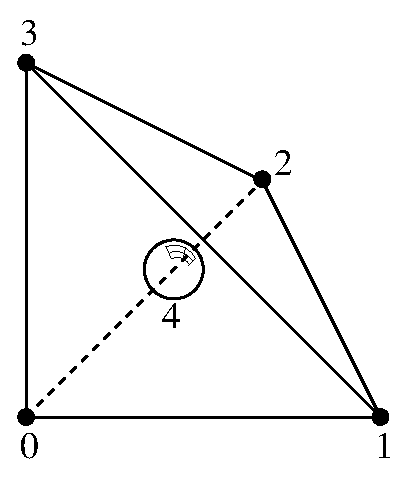
\includegraphics[width=4.5cm,angle=0]{getfemlist_tetrahedron_P1_bubble.eps} & 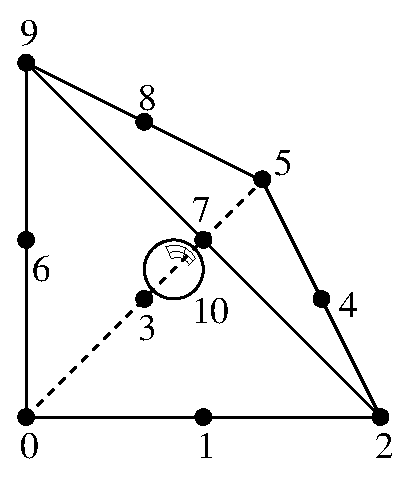
\includegraphics[width=4.5cm,angle=0]{getfemlist_tetrahedron_P2_bubble.eps} & 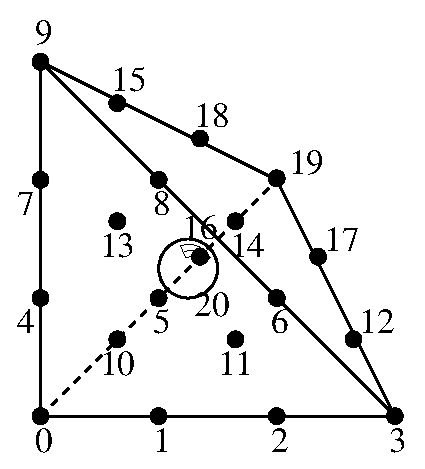
\includegraphics[width=4.5cm,angle=0]{getfemlist_tetrahedron_P3_bubble.eps}  \\
      $P_1$ with additional bubble function, 5 d.o.f., $C^0$ & $P_2$ with additional bubble function, 11 d.o.f., $C^0$ & $P_3$ with additional bubble function, 21 d.o.f., $C^0$
    \end{tabular}
  \end{center}
  \caption{ \it Lagrange element on a tetrahedron with additional internal bubble function.} 
  \label{fig:tetrahedron_p1_bubble}
\end{figure}

\begin{center}
\begin{tabular}{|m{16.11cm}|} \hline 
{ \bf $P_K$ Lagrange element with an additional internal bubble function}\\
{\tt "FEM\_PK\_WITH\_CUBIC\_BUBBLE(3, K)"} 
\end{tabular} \\ \vspace{-1pt} 
\begin{tabular}{|m{2cm}|m{2cm}|m{2.5cm}|m{1.2cm}|m{2cm}|m{2cm}|m{1.8cm}|} \hline 
Degree & dimension & d.o.f. number & class & vectorial & \mbox{$\tau$-equivalent} & Polynomial\\ \hline
$4$ & $3$ & $5$, $11$ or $21$ & $C^0$ & No \mbox{($Q = 1$)} & Yes & Yes\\ \hline
\end{tabular}
\end{center}

\begin{figure}[H]
  \begin{center}
    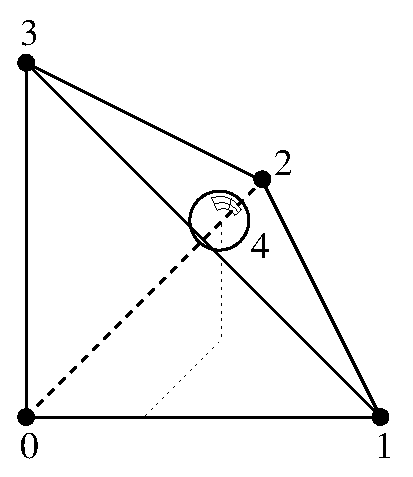
\includegraphics[width=5cm,angle=0]{getfemlist_tetrahedron_P1_bubble_face.eps}
  \end{center}
  \caption{ \it $P_1$ Lagrange element on a tetrahedron with additional bubble function on face 0, 5 d.o.f., $C^0$} 
  \label{fig:tetrahedron_p1_bubble_face}
\end{figure}

\begin{center}
\begin{tabular}{|m{16.11cm}|} \hline 
{ \bf Lagrange $P_1$ element with an additional bubble function on face 0}\\
{\tt "FEM\_P1\_BUBBLE\_FACE(3)"} 
\end{tabular} \\ \vspace{-1pt} 
\begin{tabular}{|m{2cm}|m{2cm}|m{2.5cm}|m{1.2cm}|m{2cm}|m{2cm}|m{1.8cm}|} \hline 
Degree & dimension & d.o.f. number & class & vectorial & \mbox{$\tau$-equivalent} & Polynomial\\ \hline
$3$ & $3$ & $5$ & $C^0$ & No \mbox{($Q = 1$)} & Yes & Yes\\ \hline
\end{tabular}
\end{center}

\subsubsection{Hermite element}

\begin{figure}[H]
  \begin{center}
    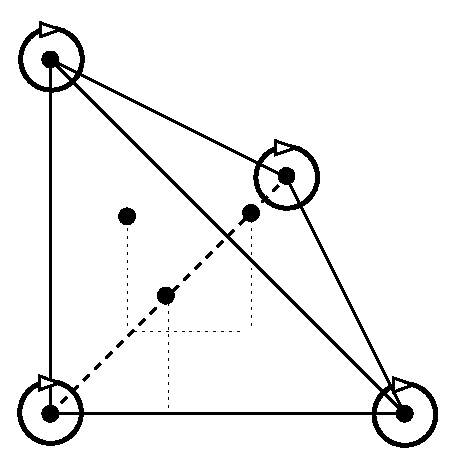
\includegraphics[width=6cm,angle=0]{getfemlist_tetrahedron_hermite.eps}
  \end{center}
  \caption{ \it Hermite element on a tetrahedron, $P_3$, 20 d.o.f., $C^0$}
  \label{fig:tetrahedron_hermite}
\end{figure}

Base functions on the reference element:
$$
  \begin{array}{ll}
\hat{\varphi}_{0}(x,y) = 1 - 3x^2 - 13xy - 13xz - 3y^2 - 13yz - 3z^2 + 2x^3 + 13x^2y + 13x^2z & \\
 ~~~~~~~~~~~~~~~ + 13xy^2 + 33xyz + 13xz^2 + 2y^3 + 13y^2z + 13yz^2 + 2z^3, & (\hat{\varphi}_0(0,0,0) = 1),\\
\hat{\varphi}_{1}(x,y) = 3x^2 - 7xy - 7xz - 2x^3 + 7x^2y + 7x^2z + 7xy^2 + 7xyz + 7xz^2, & (\hat{\varphi}_0(1,0,0) = 1),\\
\hat{\varphi}_{2}(x,y) = -7xy + 3y^2 - 7yz + 7x^2y + 7xy^2 + 7xyz - 2y^3 + 7y^2z + 7yz^2, & (\hat{\varphi}_0(0,1,0) = 1),\\
\hat{\varphi}_{3}(x,y) = -7xz - 7yz + 3z^2 + 7x^2z + 7xyz + 7xz^2 + 7y^2z + 7yz^2 - 2z^3, & (\hat{\varphi}_0(0,0,1) = 1),\\
\hat{\varphi}_{4}(x,y) = 27xyz, & (\hat{\varphi}_0(1/3,1/3,1/3) = 1),\\
\hat{\varphi}_{5}(x,y) = 27yz - 27xyz - 27y^2z - 27yz^2, & (\hat{\varphi}_0(0,1/3,1/3) = 1),\\
\hat{\varphi}_{6}(x,y) = 27xz - 27x^2z - 27xyz - 27xz^2, & (\hat{\varphi}_0(1/3,0,1/3) = 1),\\
\hat{\varphi}_{7}(x,y) = 27xy - 27x^2y - 27xy^2 - 27xyz, & (\hat{\varphi}_0(1/3,1/3,0) = 1),\\
\hat{\varphi}_{8}(x,y) = x - 2x^2 - 3xy - 3xz + x^3 + 3x^2y + 3x^2z + 2xy^2 + 4xyz + 2xz^2, & (\hat{\partial_x\varphi}_0(0,0,0) = 1),\\
\hat{\varphi}_{9}(x,y) = -x^2 + 2xy + 2xz + x^3 - 2x^2y - 2x^2z - 2xy^2 - 2xyz - 2xz^2, & (\hat{\partial_x\varphi}_0(1,0,0) = 1),\\
\hat{\varphi}_{10}(x,y) = -xy + x^2y + 2xy^2, & (\hat{\partial_x\varphi}_0(0,1,0) = 1),\\
\hat{\varphi}_{11}(x,y) = -xz + x^2z + 2xz^2, & (\hat{\partial_x\varphi}_0(0,0,1) = 1),\\
\hat{\varphi}_{12}(x,y) = y - 3xy - 2y^2 - 3yz + 2x^2y + 3xy^2 + 4xyz + y^3 + 3y^2z + 2yz^2, & (\hat{\partial_y\varphi}_0(0,0,0) = 1),\\
\hat{\varphi}_{13}(x,y) = -xy + 2x^2y + xy^2, & (\hat{\partial_y\varphi}_0(1,0,0) = 1),\\
\hat{\varphi}_{14}(x,y) = 2xy - y^2 + 2yz - 2x^2y - 2xy^2 - 2xyz + y^3 - 2y^2z - 2yz^2, & (\hat{\partial_y\varphi}_0(0,1,0) = 1),\\
\hat{\varphi}_{15}(x,y) = -yz + y^2z + 2yz^2, & (\hat{\partial_y\varphi}_0(0,0,1) = 1),\\
\hat{\varphi}_{16}(x,y) = z - 3xz - 3yz - 2z^2 + 2x^2z + 4xyz + 3xz^2 + 2y^2z + 3yz^2 + z^3, & (\hat{\partial_z\varphi}_0(0,0,0) = 1),\\
\hat{\varphi}_{17}(x,y) = -xz + 2x^2z + xz^2, & (\hat{\partial_z\varphi}_0(1,0,0) = 1),\\
\hat{\varphi}_{18}(x,y) = -yz + 2y^2z + yz^2, & (\hat{\partial_z\varphi}_0(0,1,0) = 1),\\
\hat{\varphi}_{19}(x,y) = 2xz + 2yz - z^2 - 2x^2z - 2xyz - 2xz^2 - 2y^2z - 2yz^2 + z^3, & (\hat{\partial_z\varphi}_0(0,0,1) = 1),\\
  \end{array}
$$
This element is not \mbox{$\tau$-equivalent} (The matrix $\tilde{M}$ is not equal to identity). On the real element linear combinaisons of $\hat{\varphi}_8$, $\hat{\varphi}_{12}$ and $\hat{\varphi}_{16}$ are used to match the gradient on the corresponding vertex. Idem on the orther vertices. 

\begin{center}
\begin{tabular}{|m{16.11cm}|} \hline 
{ \bf Hermite element on a tetrahedron}\\
"FEM\_HERMITE(3)"
\end{tabular} \\ \vspace{-1pt} 
\begin{tabular}{|m{2cm}|m{2cm}|m{2.5cm}|m{1.2cm}|m{2cm}|m{2cm}|m{1.8cm}|} \hline 
Degree & dimension & d.o.f. number & class & vectorial & \mbox{$\tau$-equivalent} & Polynomial\\ \hline
$3$ & $3$ & $20$ & $C^0$ & No \mbox{($Q = 1$)} & No & Yes\\ \hline
\end{tabular}
\end{center}

\subsection{Interpolation of elements on different meshes}

\begin{figure}[H]
  \begin{center}
    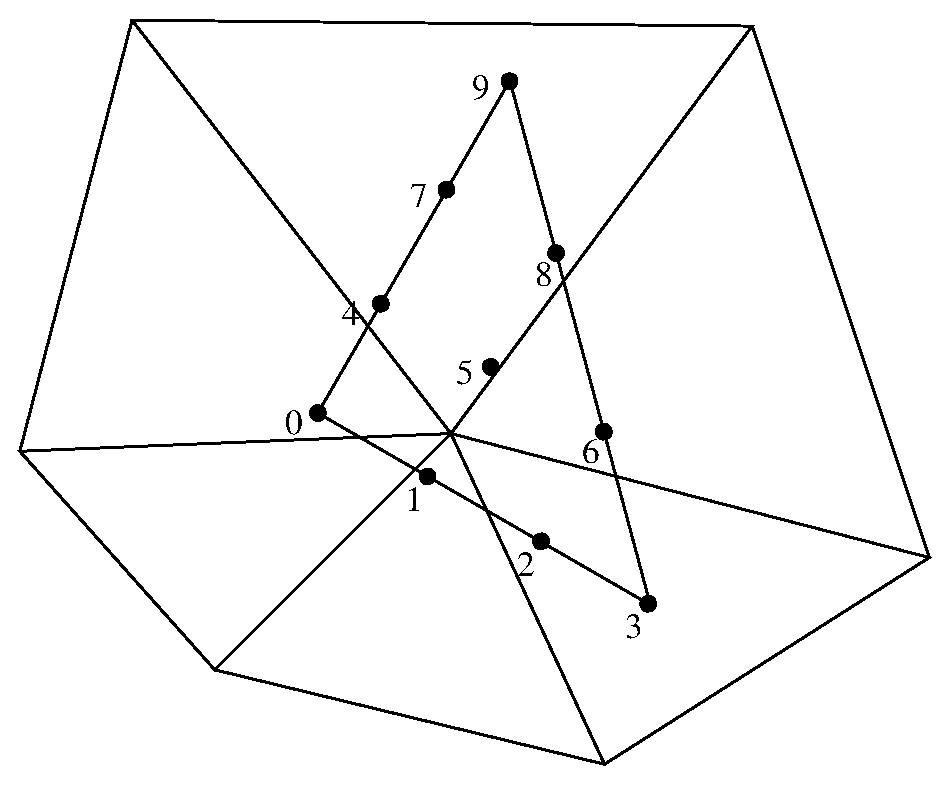
\includegraphics[width=5cm,angle=0]{getfemlist_virtual_fem.eps}
  \end{center}
  \caption{ \it Element which intepolates a finite element method defined on another mesh. The element has as many d.o.f. as the union of d.o.f. of elements of the other mesh having an intersection with it. The interpolation is made on Gauss points of the integration method.} 
  \label{fig:virtual_fem}
\end{figure}

To increase the precision, it is not necessary to raise the order of the integration method. It is recommended to keep the normal order and use composite integration methods (see below).

\begin{center}
\begin{tabular}{|m{16.11cm}|} \hline 
{ \bf Element which interpolates an element defined on another mesh}\\
  {\tt getfem::virtual\_link\_fem(getfem::mesh\_fem mf1, getfem::mesh\_fem mf2,} \\ {\tt \mbox{}\hspace{12em} getfem::pintegration\_method pim) } \\
  {\tt \mbox{}\hspace{5em} getfem::virtual\_link\_fem\_with\_gradient(getfem::mesh\_fem mf1, } \\ {\tt \hspace{5em} getfem::mesh\_fem mf2, \mbox{}getfem::pintegration\_method pim) } \\  \hline 
\end{tabular} \\ \vspace{-1pt} 
\end{center}

\section{Integration methods}

\subsection{Integration methods description}

The integration methods are of two kinds. Exact integrations of polynomials and approximated integrations (cubature formulas) of any function. The exact integration can only be used if all the elements are polynomial and if the geometric transformation is linear.

 A descriptor on an integration method is available thanks to the function\\[0.5cm]
{\tt
  ppi = getfem::int\_method\_descriptor("name of method");
}\\[0.5cm]
where {\tt "name of method"} is a string to be choosen among the existing methods.

The program \texttt{integration} located in the \texttt{tests} directory lists and checks the degree of each integration method.

\subsection{Exact Integration methods}

The list of available Exact integration methods is the following

\begin{center} \begin{tabular}{|m{0.55\linewidth}|m{0.4\linewidth}|} \hline
{\tt "IM\_EXACT\_SIMPLEX(n)"} & Description of the exact integration of polynomials on the simplex of reference of dimension {\tt n}. \\ \hline
\end{tabular}  
\begin{tabular}{|m{0.55\linewidth}|m{0.4\linewidth}|} \hline
{\tt "IM\_PRODUCT(a, b)"} & Description of the exact integration on the convex which is the direct product of the convex in {\tt a} and in {\tt b}.\\ \hline
\end{tabular}  
\begin{tabular}{|m{0.55\linewidth}|m{0.4\linewidth}|} \hline
{\tt "IM\_EXACT\_PARALLELEPIPED(n)"} & Description of the exact integration of polynomials on the parallelepiped of reference of dimension {\tt n}\\ \hline
\end{tabular}  
\begin{tabular}{|m{0.55\linewidth}|m{0.4\linewidth}|} \hline
{\tt "IM\_EXACT\_PRISM(n)"} & Description of the exact integration of polynomials on the prism of reference of dimension {\tt n}\\ \hline
\end{tabular} \end{center}


Even though a description of exact integration method exists on parallelepipeds or prisms, most of the time the geometric transformations on such elements are not linear and the exact integration cannot be used.

\subsection{Newton cotes Integration methods}

use {\tt "IM\_NC(N,K)"}, {\tt "IM\_NC\_PARALLELEPIPED(N,K)"}
and {\tt "IM\_NC\_PRISM(N,K)"} to have the Newton cotes integration of order {\tt K} respectively on simplices, parallelepipeds and prisms.


\subsection{Gauss Integration methods on dimension 1}

use {\tt "IM\_GAUSS1D(K)"} to have the Gauss-Legendre integration on the segment of order {\tt K} (with {\tt K}/2 + 1 points), and {\tt "IM\_GAUSSLOBATTO1D(K)"} to have the Gauss-Lobatto-Legendre integration on the segment of order {\tt K} (with {\tt K}/2 + 1 points). The latter integration method is only available for odd values of $K$. The Gauss-Lobatto integration method can be used in conjunction with {\tt "FEM\_PK\_GAUSSLOBATTO1D(K/2)"} to perform mass-lumping.

\subsection{Gauss Integration methods on dimension 2}

\begin{tabular}{|m{2.5cm}|m{6cm}|m{1.2cm}|m{6.5cm}|} \hline 
graphic & coordinates \hspace{5em} \begin{tabular}{m{3cm}m{3cm}} x & y  \end{tabular} & weights & function to call / order \\ \hline
\end{tabular}
\begin{tabular}{|m{2.5cm}|m{6cm}|m{1.2cm}|m{6.5cm}|}
  \hline& & &\\ 
  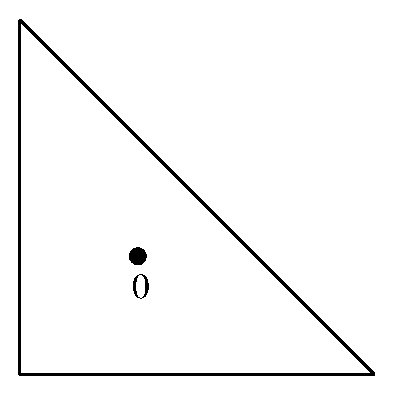
\includegraphics[width=2.5cm,angle=0]{getfemlist_intmethod_triangle1.eps} & 
  { \small
    \begin{tabular}{m{3cm}m{3cm}}
      $1/3$ & $1/3$ 
    \end{tabular}
    }
  & 
    \begin{tabular}{c}
      1/2
    \end{tabular}
  & {\tt \small "IM\_TRIANGLE(1)"} \hspace{9em} 
    1 point, order 1. \\ \hline
\end{tabular}
\begin{tabular}{|m{2.5cm}|m{6cm}|m{1.2cm}|m{6.5cm}|}
  \hline& & &\\ 
  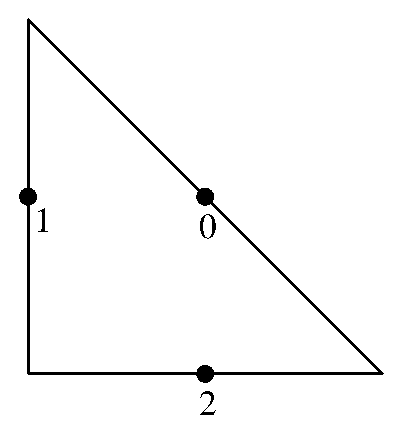
\includegraphics[width=2.5cm,angle=0]{getfemlist_intmethod_triangle2.eps} & 
  { \small
    \begin{tabular}{m{3cm}m{3cm}}
      $1/6$ & $1/6$ \\ \\
      $2/3$ & $1/6$  \\ \\
      $1/6$ & $2/3$
    \end{tabular}
    }
  & 
    \begin{tabular}{c}
      1/6 \\ \\
      1/6 \\ \\
      1/6
    \end{tabular}
  & {\tt \small "IM\_TRIANGLE(2)"} \hspace{9em} 3 points, order 2. \\ \hline
\end{tabular} 
\begin{tabular}{|m{2.5cm}|m{6cm}|m{1.2cm}|m{6.5cm}|}
  \hline& & &\\ 
  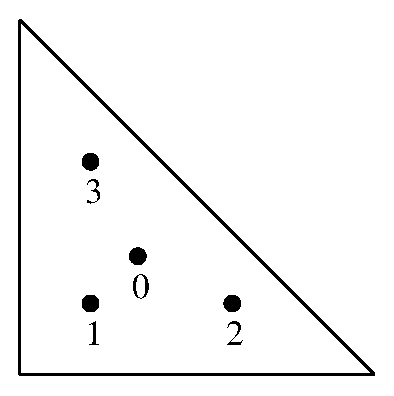
\includegraphics[width=2.5cm,angle=0]{getfemlist_intmethod_triangle3.eps} & 
  { \small
    \begin{tabular}{m{3cm}m{3cm}}
      $1/3$ & $1/3$ \\ \\
      $1/5$ & $1/5$ \\ \\
      $3/5$ & $1/5$ \\ \\
      $1/5$ & $3/5$
    \end{tabular}
    }
  & { \small
    \begin{tabular}{c}
      -27/96 \\ \\
      25/96 \\ \\
      25/96 \\ \\ 
      25/96 
    \end{tabular} }
  & {\tt \small "IM\_TRIANGLE(3)"} \hspace{9em} 4 points, order 3. \\ \hline
\end{tabular} 
\begin{tabular}{|m{2.5cm}|m{6cm}|m{1.2cm}|m{6.5cm}|}
  \hline& & &\\ 
  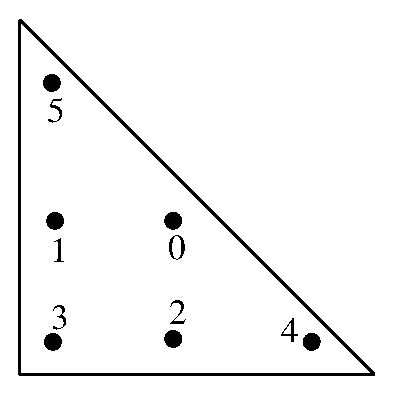
\includegraphics[width=2.5cm,angle=0]{getfemlist_intmethod_triangle4.eps} & 
  { \small
    \begin{tabular}{m{3cm}m{3cm}}
      $a$ & $a$ \\ 
      $1-2a$ & $a$ \\ 
      $a$ & $1-2a$ \\ 
      $b$ & $b$ \\ 
      $1-2b$ & $b$  \\ 
      $b$ & $1-2b$
    \end{tabular}
    }
  & { \small
    \begin{tabular}{c}
      c \\ 
      c \\ 
      c \\ 
      d \\ 
      d \\ 
      d
    \end{tabular} }
  & {\tt \small "IM\_TRIANGLE(4)"} \hspace{7em} \mbox{6 points, order 4,}\hspace{7em} \mbox{a = 0.445948490915965,}\hspace{5em} \mbox{b = 0.091576213509771,}\hspace{5em} \mbox{c = 0.111690794839005,}\hspace{5em} \mbox{d = 0.054975871827661.} \\ \hline
\end{tabular} 
\begin{tabular}{|m{2.5cm}|m{6cm}|m{1.2cm}|m{6.5cm}|}
  \hline& & &\\ 
  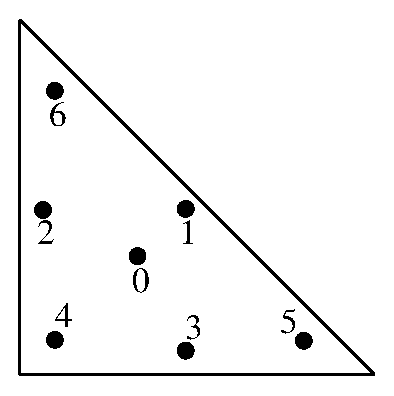
\includegraphics[width=2.5cm,angle=0]{getfemlist_intmethod_triangle5.eps} & 
  { \small
    \begin{tabular}{m{3cm}m{3cm}}
      $1/3$ & $1/3$ \\ 
      $a$ & $a$ \\ 
      $1-2a$ & $a$ \\ 
      $a$ & $1-2a$ \\ 
      $b$ & $b$ \\ 
      $1-2b$ & $b$  \\ 
      $b$ & $1-2b$
    \end{tabular}
    }
  & { \small
    \begin{tabular}{c}
      9/80 \\ 
      c \\ 
      c \\ 
      c \\ 
      d \\ 
      d \\ 
      d 
    \end{tabular} }
  & {\tt \small "IM\_TRIANGLE(5)"} \hspace{7em} \mbox{7 points, order 5,}\hspace{7em} \mbox{$a = \Frac{6+\sqrt{15}}{21}$,}\hspace{5em} \mbox{$b = 4/7 - a$,}\hspace{8em} \mbox{$c = \Frac{155+\sqrt{15}}{2400}$,}\hspace{5em} \mbox{$d = 31/240 - c$.} \\ \hline
\end{tabular}  
\begin{tabular}{|m{2.5cm}|m{6cm}|m{1.2cm}|m{6.5cm}|}
  \hline& & &\\ 
  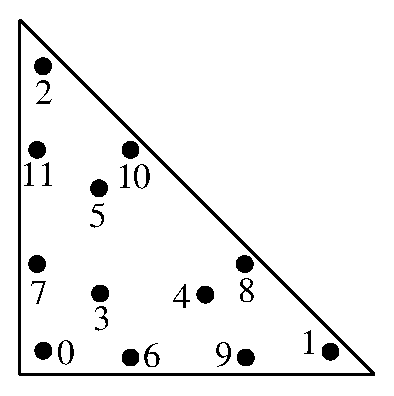
\includegraphics[width=2.5cm,angle=0]{getfemlist_intmethod_triangle6.eps} & 
  { \small
    \begin{tabular}{m{3cm}m{3cm}}
      $a$ & $a$ \\ 
      $1-2a$ & $a$ \\ 
      $a$ & $1-2a$ \\ 
      $b$ & $b$ \\ 
      $1-2b$ & $b$ \\ 
      $b$ & $1-2b$ \\ 
      $c$ & $d$ \\ 
      $d$ & $c$ \\ 
      $1-c-d$ & $c$ \\ 
      $1-c-d$ & $d$ \\ 
      $c$ & $1-c-d$ \\ 
      $d$ & $1-c-d$
    \end{tabular}
    }
  & { \small
    \begin{tabular}{c}
      e \\
      e \\ 
      e \\ 
      f \\  
      f \\ 
      f \\ 
      g \\ 
      g \\ 
      g \\ 
      g \\ 
      g \\ 
      g
    \end{tabular} }
  & {\tt \small "IM\_TRIANGLE(6)"} \hspace{7em} \mbox{12 points, order 6,}\hspace{7em}
  \mbox{$a = 0.063089104491502$,}\hspace{5em}
  \mbox{$b = 0.249286745170910$,}\hspace{8em}
  \mbox{$c = 0.310352451033785$,}\hspace{5em}
  \mbox{$d = 0.053145049844816$,}\hspace{5em}
  \mbox{$e = 0.025422453185103$,}\hspace{5em}
  \mbox{$f = 0.058393137863189$,}\hspace{5em}
  \mbox{$g = 0.041425537809187$.}\hspace{5em}
  \\ \hline
\end{tabular}  
\begin{tabular}{|m{2.5cm}|m{6cm}|m{1.2cm}|m{6.5cm}|}
  \hline& & &\\ 
  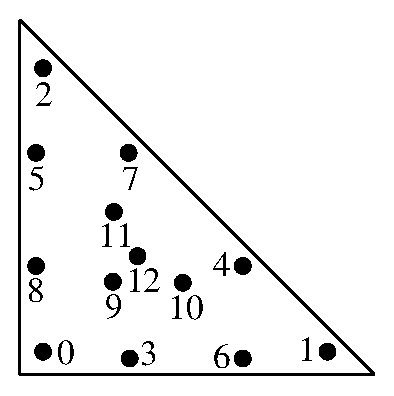
\includegraphics[width=2.5cm,angle=0]{getfemlist_intmethod_triangle7.eps} & 
  { \small
    \begin{tabular}{m{3cm}m{3cm}}
      $a$ & $a$ \\ 
      $b$ & $a$ \\ 
      $a$ & $b$ \\ 
      $c$ & $e$ \\ 
      $d$ & $c$ \\ 
      $e$ & $d$ \\ 
      $d$ & $e$ \\ 
      $c$ & $d$ \\ 
      $e$ & $c$ \\ 
      $f$ & $f$ \\ 
      $g$ & $f$ \\ 
      $f$ & $g$ \\
      $1/3$ & $1/3$ 
    \end{tabular}
    }
  & { \small
    \begin{tabular}{c}
      h \\
      h \\ 
      h \\ 
      i \\  
      i \\ 
      i \\ 
      i \\ 
      i \\ 
      i \\
      j \\
      j \\
      j \\
      k
    \end{tabular} }
  & {\tt \small "IM\_TRIANGLE(7)"} \hspace{7em} \mbox{13 points, order 7,}\hspace{7em}
  \mbox{$a = 0.0651301029022$,}\hspace{5em}
  \mbox{$b = 0.8697397941956$,}\hspace{5em}
  \mbox{$c = 0.3128654960049$,}\hspace{5em}
  \mbox{$d = 0.6384441885698$,}\hspace{5em}
  \mbox{$e = 0.0486903154253$,}\hspace{5em}
  \mbox{$f = 0.2603459660790$,}\hspace{5em}
  \mbox{$g = 0.4793080678419$,}\hspace{5em}
  \mbox{$h = 0.0266736178044$,}\hspace{5em}
  \mbox{$i = 0.0385568804451$,}\hspace{5em}
  \mbox{$j = 0.0878076287166$,}\hspace{5em}
  \mbox{$k = -0.0747850222338$.}\hspace{5em}
  \\ \hline
\end{tabular}  
\begin{tabular}{|m{2.5cm}|m{6cm}|m{1.2cm}|m{6.5cm}|} \hline
&&&{\tt \small "IM\_TRIANGLE(8)"}~(see \cite{EncyclopCubature}) \hspace{7em} \mbox{16 points, order 8}\hspace{7em} \\ \hline
\end{tabular}
\begin{tabular}{|m{2.5cm}|m{6cm}|m{1.2cm}|m{6.5cm}|} \hline
&&&{\tt \small "IM\_TRIANGLE(9)"}~(see \cite{EncyclopCubature}) \hspace{7em} \mbox{19 points, order 9}\hspace{7em} \\ \hline
\end{tabular}
\begin{tabular}{|m{2.5cm}|m{6cm}|m{1.2cm}|m{6.5cm}|} \hline
&&&{\tt \small "IM\_TRIANGLE(10)"}~(see \cite{EncyclopCubature}) \hspace{7em} \mbox{25 points, order 10}\hspace{7em} \\ \hline
\end{tabular}
\begin{tabular}{|m{2.5cm}|m{6cm}|m{1.2cm}|m{6.5cm}|} \hline
&&&{\tt \small "IM\_TRIANGLE(13)"}~(see \cite{EncyclopCubature}) \hspace{7em} \mbox{37 points, order 13}\hspace{7em} \\ \hline
\end{tabular}
\begin{tabular}{|m{2.5cm}|m{6cm}|m{1.2cm}|m{6.5cm}|}
  \hline& & &\\ 
  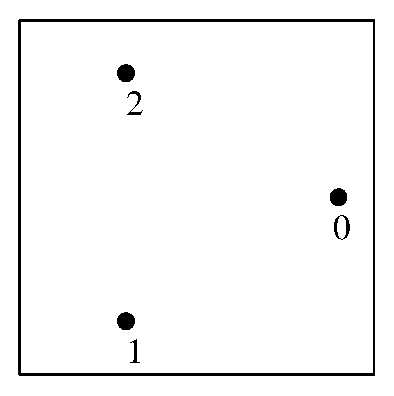
\includegraphics[width=2.5cm,angle=0]{getfemlist_intmethod_quad2.eps} & 
  { \small
    \begin{tabular}{m{3cm}m{3cm}}
      $1/2+\sqrt{1/6}$ & $1/2$ \\ \\
      $1/2-\sqrt{1/24}$ & $1/2\pm\sqrt{1/8}$ 
    \end{tabular}
    }
  & 
    \begin{tabular}{c}
      1/3 \\ \\
      1/3
    \end{tabular}
  & {\tt \small "IM\_QUAD(2)"} \hspace{11em} 3 points, order 2. \\ \hline
\end{tabular}  
\begin{tabular}{|m{2.5cm}|m{6cm}|m{1.2cm}|m{6.5cm}|}
  \hline& & &\\ 
  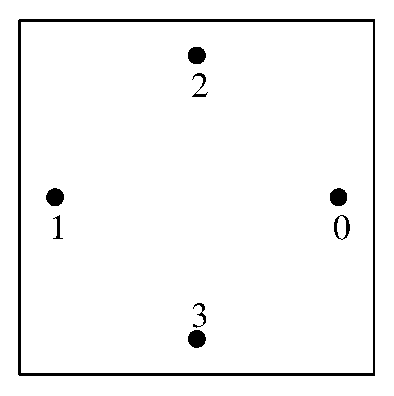
\includegraphics[width=2.5cm,angle=0]{getfemlist_intmethod_quad3.eps} & 
  { \small
    \begin{tabular}{m{3cm}m{3cm}}
      $1/2\pm\sqrt{1/6}$ & $1/2$ \\ \\
      $1/2$ & $1/2\pm\sqrt{1/6}$ 
    \end{tabular}
    }
  & 
    \begin{tabular}{c}
      1/4 \\ \\
      1/4
    \end{tabular}
  & {\tt \small "IM\_QUAD(3)"} \hspace{11em} 4 points, order 3. \\ \hline
\end{tabular} 
\begin{tabular}{|m{2.5cm}|m{6cm}|m{1.2cm}|m{6.5cm}|}
  \hline& & &\\ 
  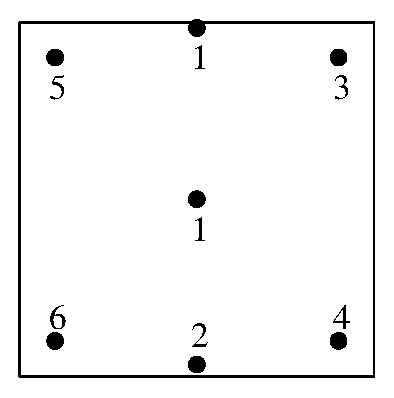
\includegraphics[width=2.5cm,angle=0]{getfemlist_intmethod_quad5.eps} & 
  { \small
    \begin{tabular}{m{3cm}m{3cm}}
      1/2 & 1/2 \\ \\
      $1/2 \pm \sqrt{7/30}$ & 1/2\\ \\
      $1/2\pm\sqrt{1/12}$ & $1/2\pm\sqrt{3/20}$ 
    \end{tabular}
    }
  & 
    \begin{tabular}{c}
      2/7 \\ \\
      5/63 \\ \\
      5/36
    \end{tabular}
  & {\tt \small "IM\_QUAD(5)"} \hspace{11em} 7 points, order 5. \\ \hline
\end{tabular}  
\begin{tabular}{|m{2.5cm}|m{6cm}|m{1.2cm}|m{6.5cm}|} \hline
&&&{\tt \small "IM\_QUAD(7)"} \hspace{7em} \mbox{12 points, order 7}\hspace{7em} \\ \hline
\end{tabular}
\begin{tabular}{|m{2.5cm}|m{6cm}|m{1.2cm}|m{6.5cm}|} \hline
&&&{\tt \small "IM\_QUAD(9)"} \hspace{7em} \mbox{20 points, order 9}\hspace{7em} \\ \hline
\end{tabular}
\begin{tabular}{|m{2.5cm}|m{6cm}|m{1.2cm}|m{6.5cm}|} \hline
&&&{\tt \small "IM\_QUAD(17)"} \hspace{7em} \mbox{70 points, order 17}\hspace{7em} \\ \hline
\end{tabular}
~\\[0.2cm]

There is also the \texttt{IM\_GAUSS\_PARALLELEPIPED(n,k)} which is a direct product of 1D gauss integrations.\\

\textbf{Important note:} do not forget that \texttt{IM\_QUAD(k)} is exact for polynomials up to degree $k$, and that a $Q_k$ polynomial has a degree of $2*k$. For example, \texttt{IM\_QUAD(7)} cannot integrate the product of two $Q_{2}$ polynomials. On the other hand, \texttt{IM\_GAUSS\_PARALLELEPIPED(2,4)} can integrate exactly that product\ldots

\subsection{Gauss Integration methods on dimension 3}

\begin{tabular}{|m{2.5cm}|m{5.5cm}|m{1.2cm}|m{7.01cm}|} \hline 
graphic & coordinates \hspace{5em} \begin{tabular}{m{1.7cm}m{1.7cm}m{1.7cm}} x & y & z \end{tabular} & weights & function to call / order \\ \hline
\end{tabular}  
\begin{tabular}{|m{2.5cm}|m{5.5cm}|m{1.2cm}|m{7.01cm}|}
  \hline& & &\\ 
  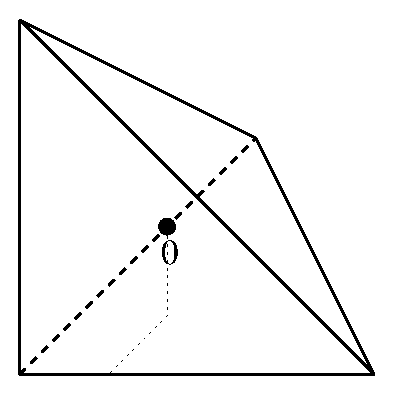
\includegraphics[width=2.5cm,angle=0]{getfemlist_intmethod_tetrahedron1.eps} & 
  { \small
    \begin{tabular}{m{1.7cm}m{1.7cm}m{1.7cm}}
      $1/4$ & $1/4$ & $1/4$  
    \end{tabular}
    }
  & 
    { \small \begin{tabular}{c}
      1/6
    \end{tabular} }
  & {\tt \small "IM\_TETRAHEDRON(1)"} \hspace{9em} 
    1 point, order 1. \\ \hline
\end{tabular}  
\begin{tabular}{|m{2.5cm}|m{5.5cm}|m{1.2cm}|m{7.01cm}|}
  \hline& & &\\ 
  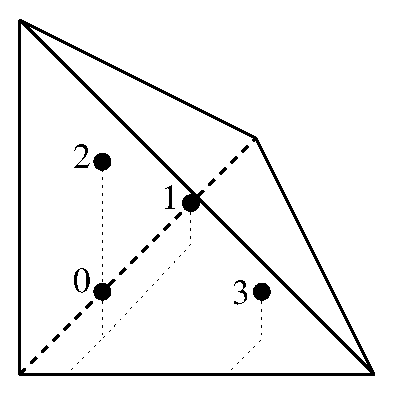
\includegraphics[width=2.5cm,angle=0]{getfemlist_intmethod_tetrahedron2.eps} & 
  { \small
    \begin{tabular}{m{1.7cm}m{1.7cm}m{1.7cm}}
      $a$ & $a$ & $a$ \\
      $a$ & $b$ & $a$ \\
      $a$ & $a$ & $b$ \\
      $b$ & $a$ & $a$ 
    \end{tabular}
    }
  & 
    { \small \begin{tabular}{c}
      1/24 \\
      1/24 \\
      1/24 \\
      1/24       
    \end{tabular} }
  & {\tt \small "IM\_TETRAHEDRON(2)"} \hspace{7em} 
    \mbox{4 points, order 2} \hspace{7em}
    \mbox{$a = \Frac{5 - \sqrt{5}}{20}$,}\hspace{5em}
    \mbox{$b = \Frac{5 + 3\sqrt{5}}{20}$.}\hspace{5em} \hspace{5em} \hspace{5em}
  \\ \hline
\end{tabular}  
\begin{tabular}{|m{2.5cm}|m{5.5cm}|m{1.2cm}|m{7.01cm}|}
  \hline& & &\\ 
  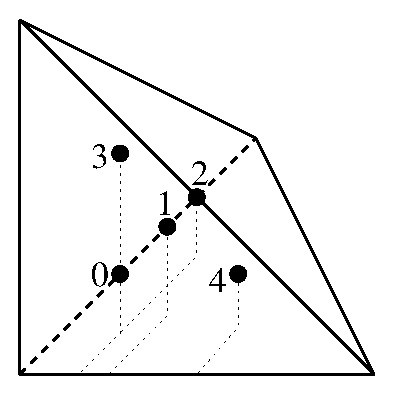
\includegraphics[width=2.5cm,angle=0]{getfemlist_intmethod_tetrahedron3.eps} & 
  { \small
    \begin{tabular}{m{1.7cm}m{1.7cm}m{1.7cm}}
      $1/4$ & $1/4$ & $1/4$ \\
      $1/6$ & $1/6$ & $1/6$ \\
      $1/6$ & $1/2$ & $1/6$ \\
      $1/6$ & $1/6$ & $1/2$ \\
      $1/2$ & $1/6$ & $1/6$      
    \end{tabular}
    }
  & 
    { \small \begin{tabular}{c}
      -2/15 \\
      3/40 \\
      3/40 \\
      3/40       
    \end{tabular} }
  & {\tt \small "IM\_TETRAHEDRON(3)"} \hspace{7em} 
    \mbox{5 points, order 3} \hspace{7em} \\ \hline
\end{tabular}  
\begin{tabular}{|m{2.5cm}|m{5.5cm}|m{1.2cm}|m{7.01cm}|}
  \hline& & &\\ 
  \includegraphics[width=2.5cm,angle=0]{getfemlist_intmethod_tetrahedron5.eps} & 
  { \small
    \begin{tabular}{m{1.7cm}m{1.7cm}m{1.7cm}}
      $1/4$ & $1/4$ & $1/4$ \\
      $a$ & $a$ & $a$ \\
      $a$ & $a$ & $c$ \\
      $a$ & $c$ & $a$ \\
      $c$ & $a$ & $a$ \\ 
      $b$ & $b$ & $b$ \\
      $b$ & $b$ & $d$ \\
      $b$ & $d$ & $b$ \\
      $d$ & $b$ & $b$ \\
      $e$ & $e$ & $f$ \\
      $e$ & $f$ & $e$ \\
      $f$ & $e$ & $e$ \\
      $e$ & $f$ & $f$ \\
      $f$ & $e$ & $f$ \\
      $f$ & $f$ & $e$ 
    \end{tabular}
    }
  & 
    { \small \begin{tabular}{c}
      8/405 \\
      h \\
      h \\
      h \\
      h \\      
      i \\
      i \\
      i \\
      i \\
      5/567 \\
      5/567 \\
      5/567 \\
      5/567 \\
      5/567 \\
      5/567
    \end{tabular} }
  & {\tt \small "IM\_TETRAHEDRON(5)"} \hspace{7em} 
    \mbox{15 points, order 5} \hspace{7em}
    \mbox{$a = \Frac{7 + \sqrt{15}}{34}$,}
    \mbox{$b = \Frac{7 - \sqrt{15}}{34}$,}\hspace{5em}
    \mbox{$c = \Frac{13 + 3\sqrt{15}}{34}$,}
    \mbox{$d = \Frac{13 - 3\sqrt{15}}{34}$,}\hspace{5em}
    \mbox{$e = \Frac{5 - \sqrt{15}}{20}$,}
    \mbox{$f = \Frac{5 + \sqrt{15}}{20}$,}\hspace{5em}
    \mbox{$h = \Frac{2665 - 14\sqrt{15}}{226800}$,}\hspace{5em} 
    \mbox{$i = \Frac{2665 + 14\sqrt{15}}{226800}$,}\hspace{5em} 
  \\ \hline
\end{tabular}

Others methods are:
\begin{center}
  \begin{tabular}{|lll|}
    \hline name & convex type & nb of points\\
    \hline \texttt{IM\_TETRAHEDRON(6)} & 3D simplex & 24\\
    \texttt{IM\_TETRAHEDRON(8)} & 3D simplex & 43\\
    \texttt{IM\_SIMPLEX4D(3)}   & 4D simplex & 6\\
    \texttt{IM\_HEXAHEDRON(5)}  & 3D parallelepipeded & 14\\
    \texttt{IM\_HEXAHEDRON(9)}  & 3D parallelepipeded & 58\\
    \texttt{IM\_HEXAHEDRON(11)}  & 3D parallelepipeded & 90\\
    \texttt{IM\_CUBE4D(5)}      & 4D parallelepipeded & 24\\
    \texttt{IM\_CUBE4D(9)}      & 4D parallelepipeded & 145\\
    \hline
  \end{tabular}
\end{center}
\subsection{Direct product of integration methods}
use {\tt "IM\_PRODUCT(IM1, IM2)"} ... for quadrilateral or prisms ... Consider using \texttt{IM\_GAUSS\_PARALLELEPIPED(2,k)}, which is an alias for \texttt{IM\_PRODUCT(IM\_GAUSS1D(2,k),IM\_GAUSS1D(2,k))} instead of the \texttt{IM\_QUAD} integrations.

\subsection{Composite integration methods}

\begin{figure}[H]
  \begin{center}
    \includegraphics[width=5cm,angle=0]{getfemlist_intmethod_triangle2_comp.eps}
  \end{center}
  \caption{ \it composite method {\tt "IM\_STRUCTURED\_COMPOSITE(IM\_TRIANGLE(2), 3)"}} 
  \label{fig:triangle_comp}
\end{figure}


use {\tt "IM\_STRUCTURED\_COMPOSITE(IM1, S)"} to copy {\tt IM1} on an element with {\tt S} subdivisions. The resulting integration method has the same order but with more points. This could be more stable to use composite method rather than to improve the order of the method. Those methods have to be used also with composite elements. Most of the time for composite element, it is preferable to choose the basic method {\tt IM1} with no points on the boundary (because the gradient coulb be not defined on the boundary of sub-elements). 

\begin{thebibliography}{99}

\bibliographystyle{apalike}
% \bibliographystyle{plain}
% \bibliography{all}
\bibitem{dh-to1984} 
  G. {\sc Dhatt, and  G. Touzot}
  {\it The Finite Element Method Displayed}, 
 J. Wiley \& Sons,  New York, 1984.

\bibitem{BAS_COMP}
  Y. {\sc Renard},
  {\it Elementary Computations in {\sc Getfem++}}, 2002.

\bibitem{USER_DOC}
  Y. {\sc Renard}, J. {\sc Pommier},
  {\it Short User Documentation of {\sc Getfem++}}, 2003.

\bibitem{nedelec1991}
  J.-C. {\sc Nedelec},
  {\it Notions sur les techniques d'{\'e}l{\'e}ments finis}, Ellipses, SMAI, Math{\'e}matiques \& Applications n$^o7$, 1991.

\bibitem{EncyclopCubature}
  R. {\sc Cools}
  {\it An Encyclopaedia of Cubature Formulas}, J. Complexity, {\tt http://www.cs.kuleuven.ac.be/{\~n}ines/research/ecf/ecf.html}

\bibitem{so-se-do2004}
  P. {\sc Solin, K. Segeth, I. Dolezel},
  {\it Higher-Order Finite Element Methods}, Chapman and Hall/CRC, Studies in advanced mathematics, 2004.


\end{thebibliography}


\end{document}
